
\section{Présentation générale du rugosimètre à grande vitesse}
\ifprof
\else
La rugosimétrie est la mesure de l’état de surface des pièces mécaniques. L’ordre de grandeur des défauts
mesurés est le micron. Cette mesure des états de surfaces est aussi répandue et indispensable que la mesure
des caractéristiques dimensionnelles et géométriques des pièces mécaniques (longueur, orientation,
perpendicularité…). La \autoref{fig_01} représente un relevé rugosimétrique tridimensionnel d’une partie d’une
aube de turbine de haute précision (à droite en fausses couleurs).


\begin{figure}[H]
\centering
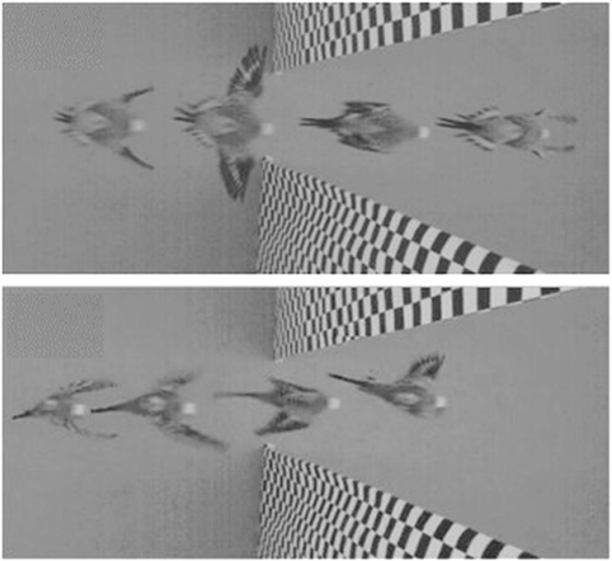
\includegraphics[width=.6\linewidth]{fig_01}
\caption{\label{fig_01} Relevé rugosimétrique tridimensionnel d’une aube}
\end{figure}

La mesure de rugosimétrie repose traditionnellement sur deux éléments distincts : le capteur, qui peut être
mécanique (palpeur) ou optique, et le traitement du signal et des données (algorithmes informatiques), qui
permet de traduire les mesures physiques de base, produites par le capteur, en données numériques
exploitables, représentatives des caractéristiques physiques de la surface analysée.


De la conjonction des caractéristiques techniques du capteur et du traitement numérique vont découler les
qualités essentielles du rugosimètre : sa rapidité ; sa résolution ; sa précision ; son amplitude de mesure.

Lorsque l’ensemble est suffisamment rapide, il peut être utilisé pour réaliser des relevés de surface
($z$ fonction de $(x, y)$, ou « mesure 3D ») et non plus simplement des profils linéaires ($z$ fonction de $x$, ou
« mesure 2D »). Si, à cette exigence de rapidité, on ajoute celle de précision ainsi que celle de grande
amplitude de mesure, on arrive, avec les technologies actuellement disponibles, à des capteurs très chers
(de l’ordre de 50 000 euros). Cela fait que le développement de la rugosimétrie 3D de précision a été,
jusqu'à présent, assez lent. Le projet, dont est tiré le sujet, a pour ambition de développer et de mettre sur le
marché un rugosimètre 3D de précision à faible coût.

L’objet de cette étude est de valider / critiquer / améliorer certaines techniques et technologies retenues
pour le prototype du rugosimètre 2D. Ce prototype a été conçu par le laboratoire SATIE de l’École
Normale Supérieure de Cachan. Ce projet est le fruit d’un travail pluridisciplinaire qui a impliqué des
commerciaux, des scientifiques et des techniciens, et a été financé par l’Agence pour la Valorisation de la
Recherche d’Ile-de-France.
\fi
\subsection{Structure générale du rugosimètre à grande vitesse}
\ifprof
\else
Le principe d’un capteur opto-mécanique (association d’un capteur optique et d’un capteur mécanique) a
été retenu, pour ce prototype. Il est décrit succinctement ci-après (\autoref{fig_02}) :
\begin{itemize}
\item un capteur optique assure une résolution verticale comparable à celle des meilleurs capteurs mécaniques actuels ($< \SI{10}{nm}$). Ce capteur, de faible amplitude de lecture (\SI{20}{\mu m}), permet une mesure rapide des hautes fréquences spatiales (variations rapides) des profils rugosimétriques mesurés ;
\item un asservissement mécanique vertical à grande amplitude (environ \SI{10}{mm}) permet à la tête optique de suivre les moyennes et basses fréquences spatiales (variations plus lentes) des profils. Un second capteur donne la position verticale de la tête optique.
\end{itemize}


\begin{figure}[H]
\centering
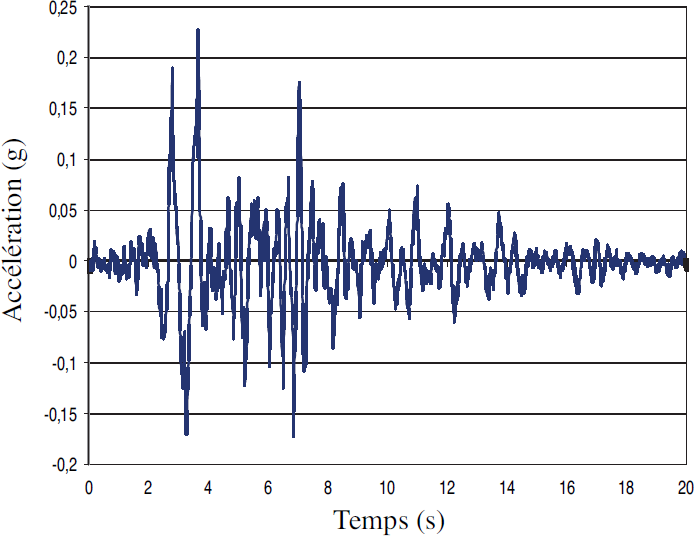
\includegraphics[width=.45\linewidth]{fig_02}
\caption{\label{fig_02} Principe du système opto-mécanique}
\end{figure}

Le profil complet sera obtenu par la somme des signaux fournis par les deux capteurs. Le déplacement
vertical du capteur optique est assuré par une Unité de Rotation (U.R.) portée par le coulisseau (2)
(\autoref{fig_03}).

\begin{figure}[H]
\centering
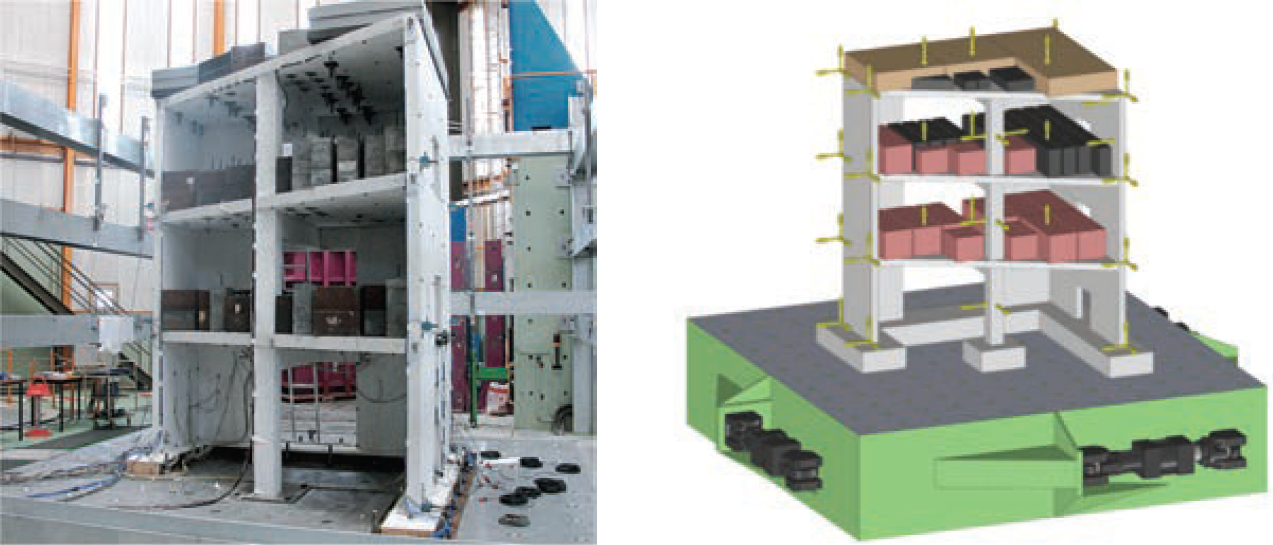
\includegraphics[width=.8\linewidth]{fig_03}
\caption{\label{fig_03} Schéma du prototype de rugosimètre 2D}
\end{figure}

Ce capteur opto-mécanique est lui-même déplacé au dessus de la surface à mesurer par une Unité de
Translation (U.T.) à vitesse régulée (\autoref{fig_03}), ce qui permet d’obtenir un « profil 2D », $z$ fonction de $x$. La
vitesse de déplacement visée par ce prototype est de \SI{20}{mm.s^{-1}}.

Dans sa future version 3D, une seconde U.T. de direction ($\vect{y}$) permettra de donner une image de la surface
par une juxtaposition de profils 2D : on « scannera » la surface.

Le coût estimé de ce rugosimètre est de 10 000 euros.
\fi
\subsection{Principe de mesure du capteur optique}
\ifprof
\else
Le principe de mesure du capteur optique est l’écartométrie. Ce procédé, déjà utilisé en robotique, n’a encore jamais servi en rugosimétrie industrielle. Un faisceau laser (« émission ») est focalisé sur la surface à mesurer. La tache focale se déplace devant les images de deux demi-disques de réception. L’intensité lumineuse d’émission se partage ainsi entre deux photorécepteurs.

Cette différence d’intensité permet de calculer la position horizontale de la tache focale d’émission. Cette position horizontale de la tache focale est ensuite convertie en position verticale de la surface par rapport au point focal (qui sera noté par la suite (P)) (\autoref{fig_04}).

\begin{figure}[H]
\centering
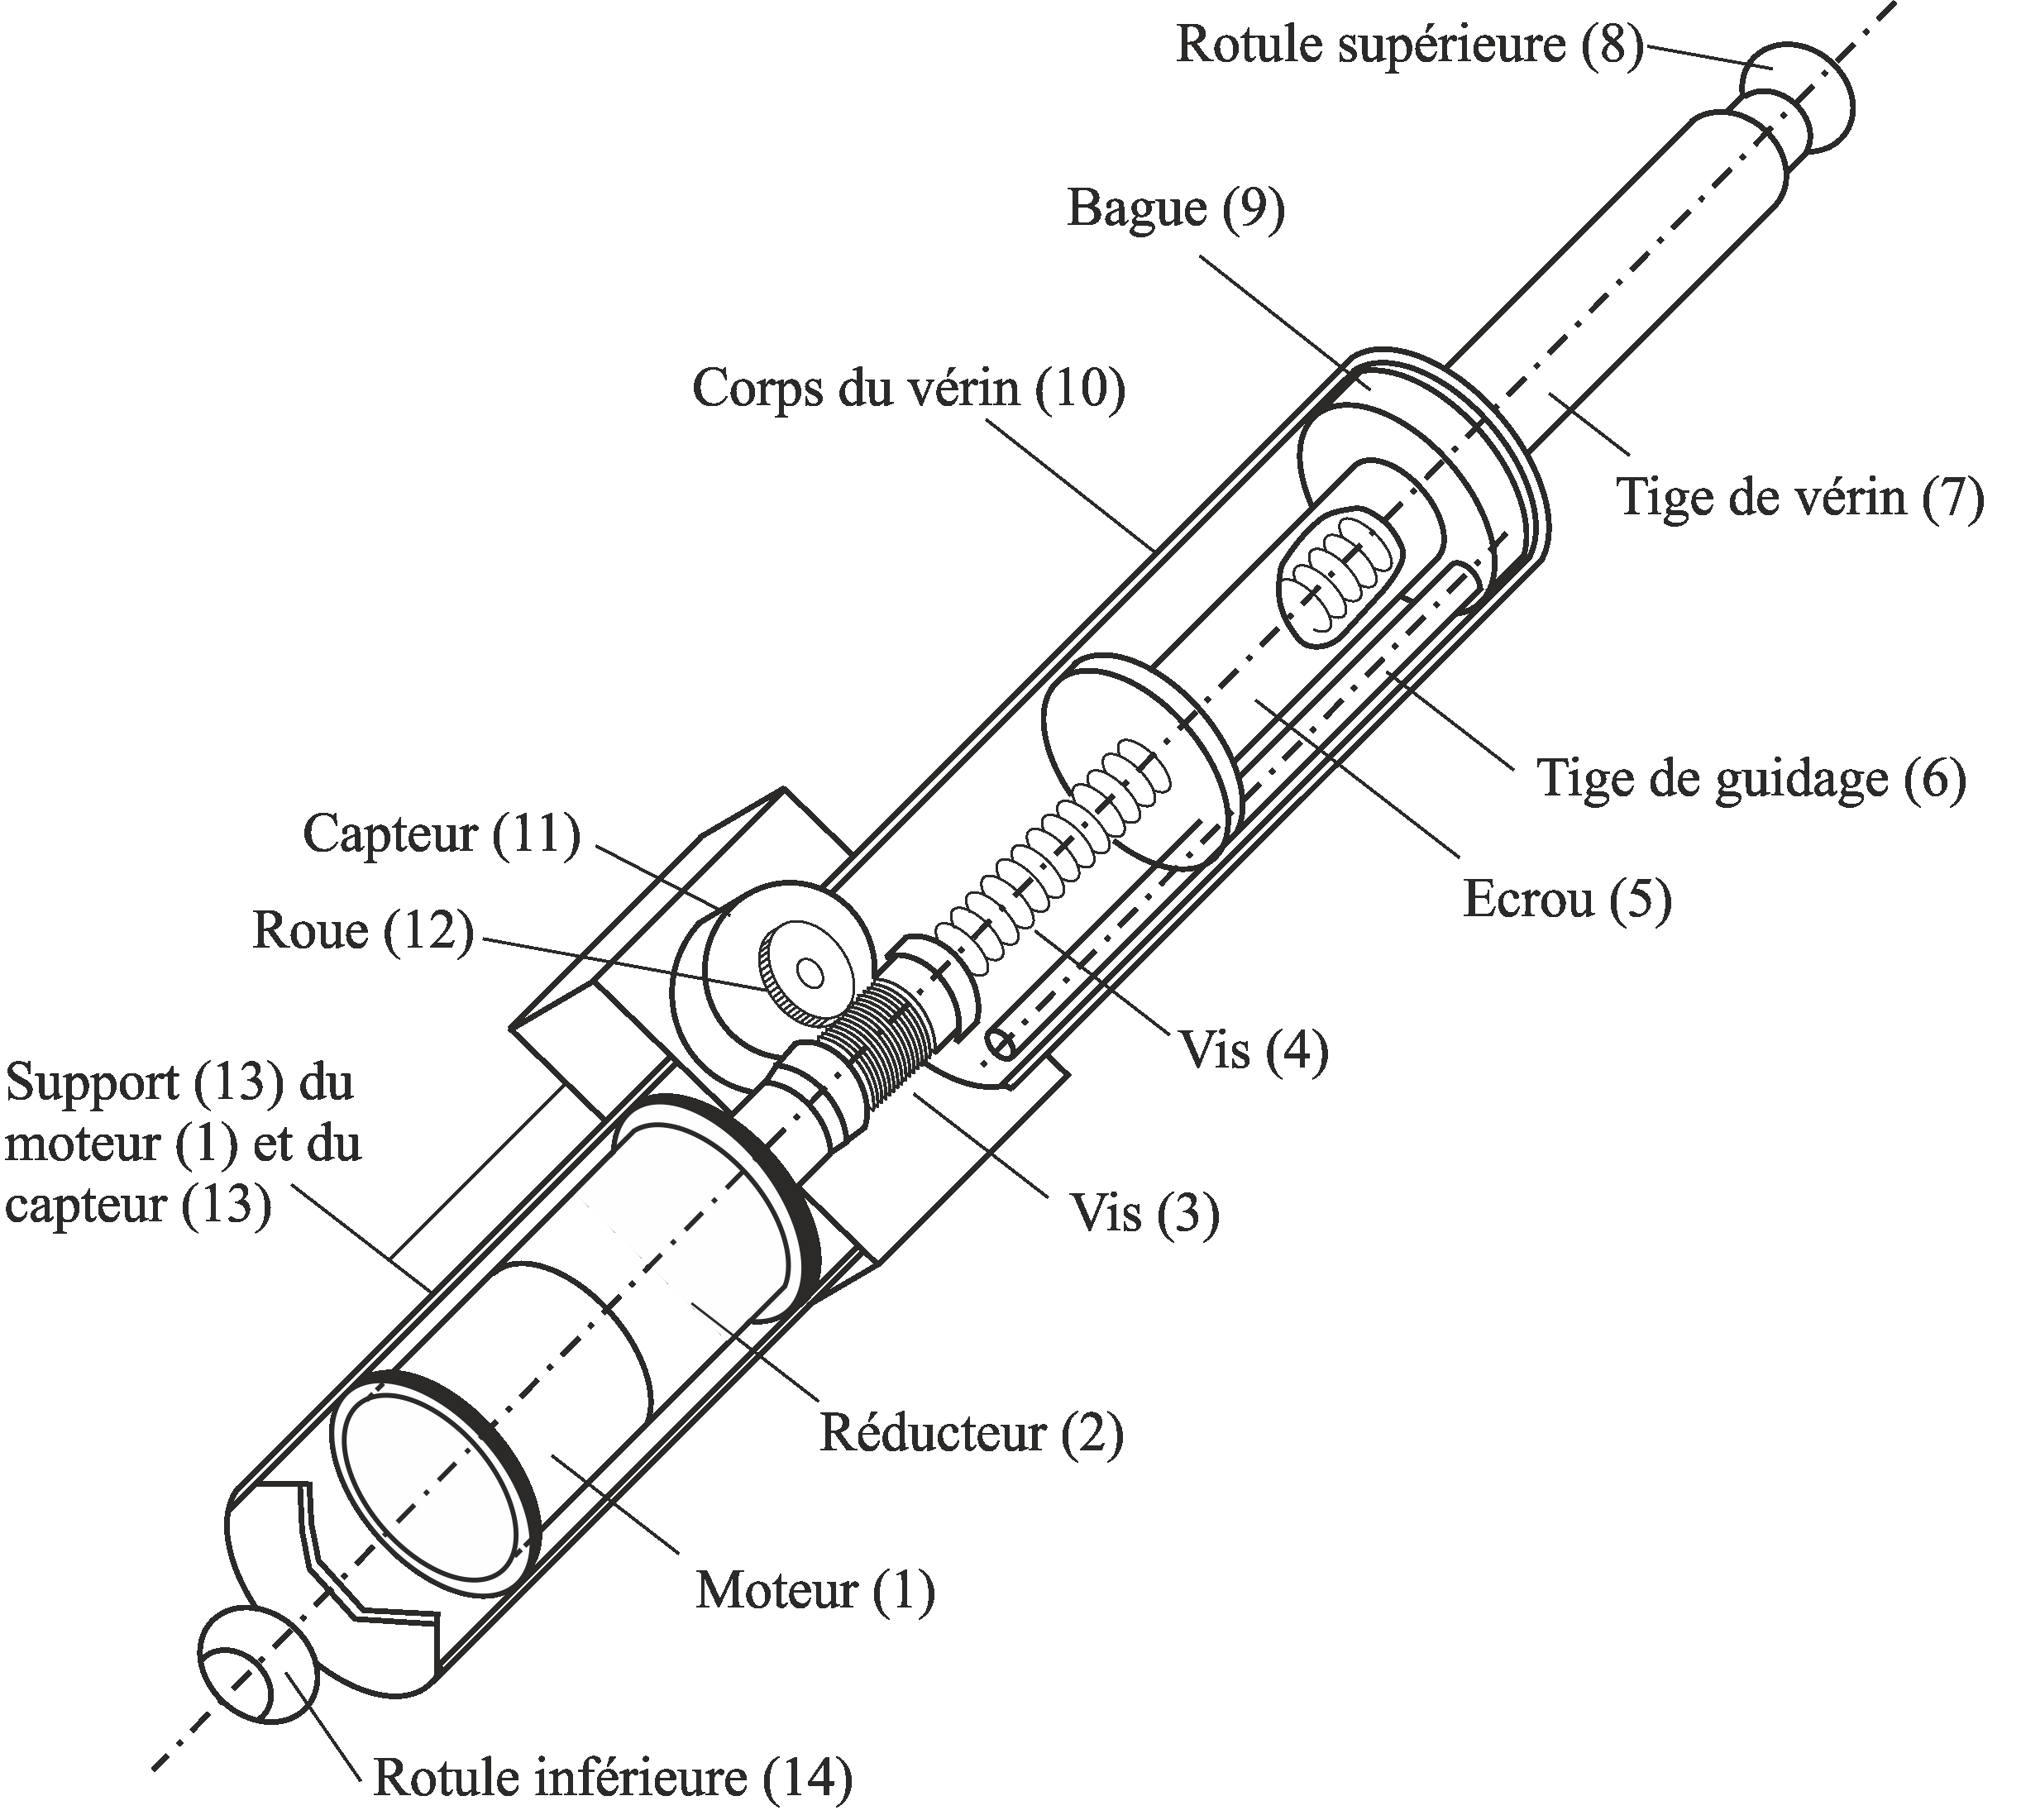
\includegraphics[width=.5\linewidth]{fig_04}
\caption{\label{fig_04} Principe du capteur optique : l’écartométrie}
\end{figure}
\fi

\section{Caractérisation globale du rugosimètre}
\ifprof
\else
Dans cette partie, nous vous demandons de caractériser de façon globale le système étudié puis de
déterminer les liens existant entre les différents éléments de ce système. Ceci permettra d’étudier
ultérieurement les caractéristiques de certains constituants, puis de les modifier si leur comportement ne
donne pas satisfaction en ayant en permanence à l’esprit les contraintes qui lient ces éléments spécifiques
aux autres éléments du système global.

Le marché économique d’un tel instrument de mesure est très concurrentiel. Les acheteurs potentiels de ces
capteurs choisissent plusieurs critères pour évaluer les différentes propositions commerciales qui peuvent
leur être faites.

\fi

\question{\label{q_01}Donner les différents critères de performance et les niveaux associés du rugosimètre.}
\ifprof
\begin{corrige} ~\\

\begin{center}
\begin{tabular}{ll}
\hline
Critères de performances & Niveaux associés \\ \hline \hline
Résolution verticale du capteur optique & $< \SI{10}{nm}$ \\ \hline
Amplitude de lecture & $\SI{20}{\mu m}$ \\ \hline
Amplitude de l'asservissement (??) & $\SI{10}{mm}$ \\ \hline
Vitesse de déplacement & $\SI{20}{mm.s^{-1}}$\\ \hline
\end{tabular}
\end{center}
\end{corrige}
\else
\fi

%\question{\label{q_02}Complétez les diagrammes S.A.D.T. « A-0 », puis « A.0 », du système « rugosimètre 3D » préfiguré par le prototype 2D décrit ci-dessus. Vous éviterez les confusions entre entrées, moyens et contrôles.}

\section{Calculs prévisionnels des actionneurs \label{sec:3}}

\ifprof
\else
Les calculs d’avant projet doivent permettre de dimensionner les différents composants qui seront utilisés
et de définir certains paramètres de réglages (paramètres d’asservissement…).

Les calculs prévisionnels visent, dans un premier temps, à déterminer les équations dynamiques qui
permettront de déterminer les couples moteurs (minimum) des différents actionneurs en fonction des
caractéristiques géométriques, massiques et inertielles des pièces ainsi que des conditions d’utilisation.

Dans toute cette partie, nous considérerons que seules l'unité de translation ($\vect{x}$ ) et l’unité de rotation sont
actionnées.
\fi

\subsection{Mise en place du problème}

\ifprof
\else
\begin{figure}[H]
\centering
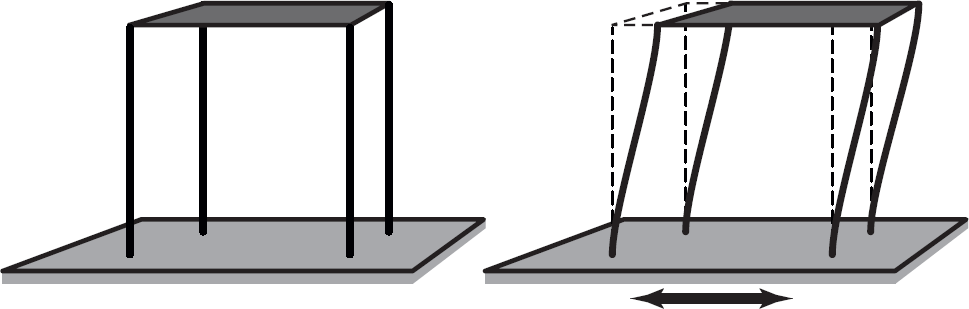
\includegraphics[width=.8\linewidth]{fig_05}
\caption{\label{fig_05} Schéma paramétré du prototype de rugosimètre 2D (les actionneurs ne sont pas représentés)}
\end{figure}

La figure 5 présente le schéma et le paramétrage qui sera utilisé pour cette partie de l’étude. Ce système
comporte quatre pièces :
\begin{itemize}
\item le bâti (0). On associe à cette pièce le repère ($\mathcal{R}_0\left(O, \vect{x_0}, \vect{y_0}, \vect{z_0}\right)$) que l’on considère galiléen ;
\item le rotor (1) :
\begin{itemize}
\item moment d’inertie selon l’axe $\left(O,\vect{x_0}\right)$  noté $J_1$ avec $J_1 = \SI{1e-6}{kg.m^2}$;
\item centre d’inertie ($G_1$), avec $\vect{OG_1} = -a\vect{x_0}$;
\item la liaison pivot ($L_{0/1}$), dont le paramètre angulaire est $\varphi = \left(\vect{y_0},\vect{x_0}\right)$, présente un frottement visqueux de coefficient $f_1$, créant un moment : $\vectm{O}{0}{1} = -f_1 \dot{\varphi} \vect{x_0}$ ($f_1 = \SI{5e-5}{Nm.rad^{-1}.s}$);
\item un moteur (M1) gère le mouvement de rotation de (1) par rapport à (0). Le couple moteur
appliqué sur (1) est noté : $\vect{C}_{\text{Moteur 1}\rightarrow 1}=C_{m1}\vect{x_0}$;
\end{itemize}
\item le coulisseau (2) :
\begin{itemize}
\item masse : $m_2$ avec $m_2 = \SI{2}{kg}$ ;
\item centre d’inertie ($G_2$),
\item la liaison hélicoïdale ($L_{1/2}$) (supposée parfaite) possède un pas noté ($p_a$) ($p_a = \SI{0,5}{mm/tour}$).
Ce pas est à droite (sens classique) ;
\item la liaison glissière ($L_{0/2}$), dont le paramètre de position (translation) est noté ($x$) : $\vect{OA} = x\vect{x_0}$, présente un frottement visqueux de coefficient $f_2$, créant une force : $\vectf{0}{2}=-f_2 \dot{x}\vect{x_0}$ ($f_2 = \SI{5}{N.m^{-1}.s}$);
\end{itemize}
\item l’ensemble (3) :
\begin{itemize}
\item masse : $m_3$ (cette masse sera déterminée à la question \ref{q_03}) ;
\item centre d’inertie ($G_3$) : $\vect{AG_3}=r\vect{x_3}$;
\item matrice d’inertie en (A) : $\inertie{A}{3} = \matinertie{A}{B}{C}{-D}{-E}{-F}{A,\mathcal{B}_3}$, avec $\mathcal{B}_3=\left(\vect{x_3},\vect{y_3},\vect{z_3}\right)$
\item la liaison pivot ($L_{2/3}$), de paramètre angulaire $\theta = \left(\vect{x_0} , \vect{x_3}\right)$, présente un frottement visqueux de coefficient $f_3$, créant un moment : $\vectm{A}{2}{3} = -f_3 \dot{\theta} \vect{y_0}$;
\item un moteur (M3) gère la rotation de l’ensemble (3) par rapport à (2). Le couple moteur appliqué
sur (3) est noté : $\vect{C}_{\text{Moteur 3}\rightarrow 3}=C_{m3}\vect{y_0}$;
\item un système d’équilibrage (ressort de torsion) permet à la tête optique d’être horizontale ($\theta = 0\degres$)
en position de repos, c’est-à-dire lorsque le moteur (M3) n’est pas alimenté. Ce système
d’équilibrage exerce sur l’ensemble (3) un couple de rappel noté : $\vect{C}=C_r \vect{y_0}$, avec
$C_r = -\left(K_{\text{tors}}\theta + C_0\right)$. Le terme $C_0$ permet d’équilibrer le moment en (A) créé par l’action de
pesanteur sur (3) lorsque ($\theta = 0\degres$).
\end{itemize}
\end{itemize}
\fi
\subsection{Positionnement du centre d'inertie}


\ifprof
\else
Comme le montre la \autoref{fig_06}, l’ensemble (3) est constitué de plusieurs solides en liaison encastrement :
\begin{itemize}
\item le bras (4) lié au moteur couple;
\item la tête optique (5);
\item un contrepoids (6).
\end{itemize}
Ce contrepoids (6) a été ajouté pour assurer que le centre d’inertie ($G_3$) soit sur l’axe $\axe{A}{x_3}$.

\begin{figure}[H]
\centering
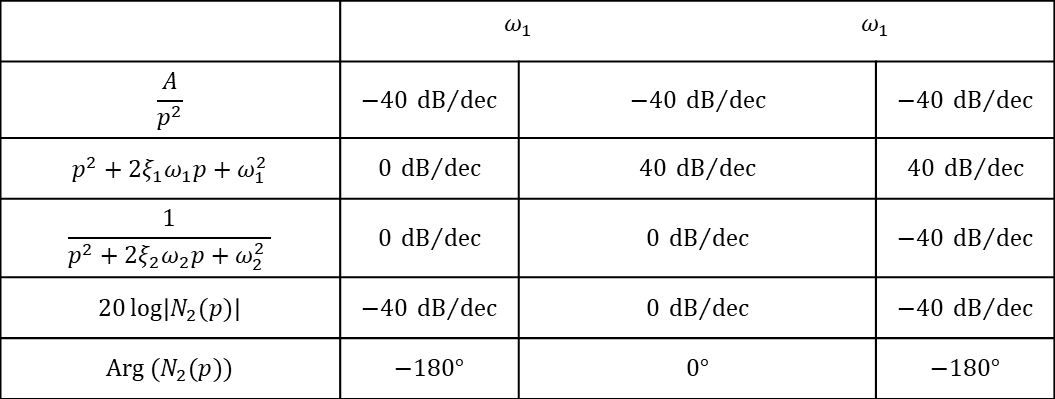
\includegraphics[width=.4\linewidth]{fig_06}
\caption{\label{fig_06} Unité de rotation}
\end{figure}

Les caractéristiques géométriques de l’ensemble (3) étudié sont données ci-après :
\begin{itemize}
\item bras (4) du moteur couple : masse : $m_4=\SI{e-3}{kg}$; centre d’inertie : $\vect{AG_4} = - b_4 \vect{y_0}$ avec $b_4 =  \SI{4}{mm}$;
\item tête optique (5) : masse : $m_5= \SI{5e-3}{kg}$; centre d’inertie : $\vect{AG_5}= a_5 \vect{x_3}+b_5 \vect{y_3}-c_5 \vect{z_3}$ avec $a_5 = \SI{40}{mm}$ ; $b_5 = \SI{0,8}{mm}$ ; $c_5 = \SI{10}{mm}$;
\item contrepoids (6) : masse : $m_6$ (à déterminer à la question \ref{q_03}) ; centre d’inertie :
$\vect{AG_6}= a_6 \vect{x_3}+c_6 \vect{z_3}$ avec $a_6 = \SI{10}{mm}$ ; $c_6 = \SI{25}{mm}$.
\end{itemize}
\fi

\question{\label{q_03}Déterminez l’expression littérale de la masse du contrepoids (6) qui assure que le terme (c) de l’expression de la position du centre d’inertie ($\vect{AG_3}=r\vect{x_3} - b\vect{y_3} + c\vect{z_3}$) est nul. Réalisez l’application numérique. Montrez que dans ce cas, $r=\SI{27,5}{mm}$ avec $\vect{AG_3}=r\vect{x_3}$.}
\ifprof
\begin{corrige} ~\\
\begin{minipage}[c]{.7\linewidth}
Déterminons la position du centre d'inertie de l'ensemble (3) en utilisant le barycentre des centres d'inertie des pièces qui le compose.

$\left(m_4 + m_5 +m_6 \right) \vect{AG_3} = m_4 \vect{AG_4}+m_5 \vect{AG_5}+m_6 \vect{AG_6} $. 

On souhaite que  $\vect{AG_3}\cdot \vect{z_3}$ soit nul. En conséquences, 
$ m_4 \vect{AG_4} \cdot \vect{z_3}+m_5 \vect{AG_5}\cdot \vect{z_3}+m_6 \vect{AG_6}\cdot \vect{z_3} = 0 $. 

On a alors :$ - m_4 b_4 \vect{y_0} \cdot \vect{z_3} - m_5 c_5 +m_6 c_6  = 0 $
$\Leftrightarrow  - m_5 c_5 +m_6 c_6  = 0 $.
$\Leftrightarrow   m_6   = m_5 \dfrac{c_5}{c_6}$.
 
\textit{Application numérique : } $m_6 = \dfrac{5\times 10^{-3} \times 10}{25} = \SI{2e-3}{kg}$.

\end{minipage} \hfill
\begin{minipage}[c]{.25\linewidth}
\begin{center}
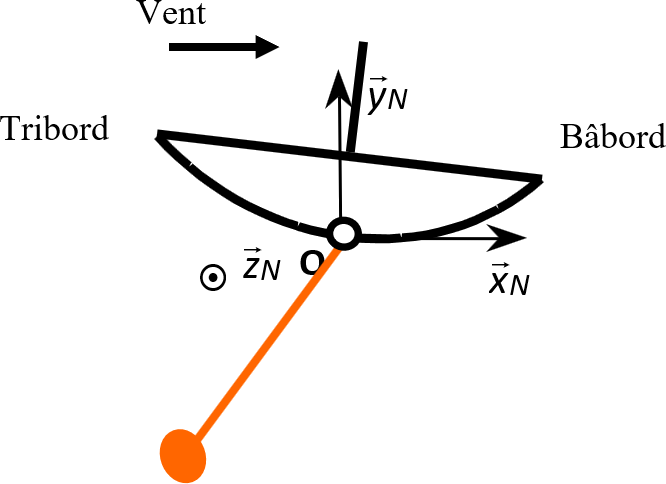
\includegraphics[width=\linewidth]{cor_01}
\end{center}
\end{minipage}

Par ailleurs, on cherche $r_3$; donc
$\left(m_4 + m_5 +m_6 \right) \vect{AG_3}\cdot \vect{x_3} = m_4 \vect{AG_4}\cdot \vect{x_3}+m_5 \vect{AG_5}\cdot \vect{x_3}+m_6 \vect{AG_6}\cdot \vect{x_3} $  
soit 
$\left(m_4 + m_5 +m_6 \right) r =m_5 a_5+m_6 a_6 $; donc $ r =\dfrac{m_5 a_5+ m_6a_6}{m_4 + m_5 +m_6 } $.

\textit{Application numérique : } $r = \dfrac{\num{5e-3}\times 40 + \num{2e-3}\times 10}{\num{e-3}+ \num{5e-3} + \num{2e-3}} = \dfrac{220}{8}=\SI{27,5}{mm}$.

Pour finir, il faudrait vérifier que $b=\SI{0}{mm}$.
\end{corrige}
\else
\fi
\subsection{Équations dynamiques}

\ifprof
\else
Le système étudié possède deux mobilités, il est donc nécessaire de déterminer deux équations pour
pouvoir atteindre les grandeurs recherchées, le couple moteur dans l’actionneur de l’unité de rotation
($C_{\text{m3}}$) et le couple moteur dans l’unité de translation ($C_{\text{m1}}$) en fonction des caractéristiques
dimensionnelles et matérielles des pièces, des lois de mouvement et des dissipations dans les liaisons.
\fi

%Pour obtenir la première équation, vous êtes obligé d’appliquer la méthode demandée.

\question{\label{q_04}Isoler l’ensemble (3) et réaliser le BAME puis écrire le théorème du moment dynamique en (A) en projection sur $\vect{y_0}$. Écrire votre résultat sous le forme $d\ddot{\theta}+e\ddot{x}+f\dot{\theta}+g\theta = h $ (les termes $d$, $e$, $f$, $g$ et $h$ peuvent dépendre de $\theta$).}
\ifprof
\begin{corrige} ~\\
\begin{itemize}
\item On isole 3.

\item Bilan des actions mécaniques extérieures.
\begin{itemize}
\item Action de la liaison pivot de (2) sur (3) 	avec frottement visqueux : $\torseurstat{T}{2}{3}$ tel que $\vectm{A}{2}{3} \cdot \vect{y_3} =  -f_3 \dot{\theta} $.
\item Action du moteur entre (2) et (3) : $\torseurstat{T}{2_{\text{m}}}{3}$ tel que $\vectm{A}{2_{\text{m}}}{3} \cdot \vect{y_3} = C_{\text{m3}} $. 
\item Action du ressort entre (2) et (3) : $\torseurstat{T}{2_{\text{r}}}{3}$ tel que $\vectm{A}{2_{\text{r}}}{3} \cdot \vect{y_3} = C_{\text{r}}= -\left(K_{\text{tors}}\theta + C_0\right) $. 
\item Action de pesanteur sur (3) : $\torseurstat{T}{\text{pes}}{3} = \torseurl{-m_3g \vect{z_0}}{\vect{0}}{G_3}$ avec 
$\vectm{A}{\text{pes}}{3} \cdot \vect{y_3} = \left(\vect{AG_3} \wedge -m_3g \vect{z_0} \right) \cdot \vect{y_3}$
$= \left(r  \vect{x_3} \wedge -m_3g \vect{z_0} \right) \cdot \vect{y_3}$
$= -rm_3g\left(  \vect{y_3} \wedge \vect{x_3} \right) \cdot \vect{z_0} $
$= rm_3g\vect{z_3} \cdot \vect{z_0} $
$= rm_3g\cos \theta $.
\end{itemize}

\item Calcul de $\vectmd{A}{3}{0}\cdot \vect{y_3} = \deriv{\vectmc{A}{3}{0}}{\rep{0}}\cdot \vect{y_3} + m_3 \left(\vect{V(A/0)}\wedge\vectv{G_3}{3}{0}\right)\cdot \vect{y_3}$.
\begin{itemize}

\item  $\deriv{\vectmc{A}{3}{0}}{\rep{0}}\cdot \vect{y_3} =  \deriv{\vectmc{A}{3}{0}\cdot \vect{y_3}}{}+ \underbrace{\vectmc{A}{3}{0}\cdot \deriv{\vect{y_3}}{\rep{0}}}_{0}$.  

\item De plus $\vectmc{A}{3}{0} = \inertie{A}{3} \vecto{3}{0}  + m_3 \vect{AG_3}\wedge \vectv{A}{3}{0}$ 
$= \matinertie{A}{B}{C}{-D}{-E}{-F}{A,\mathcal{B}_3} \begin{pmatrix} 0  \\ \dot{\theta} \\ 0 \end{pmatrix}_{\rep{3}}
+ m_3 r\vect{x_3}\wedge \dot{x}\vect{x_0} $ 

$ =\begin{pmatrix} -F\dot{\theta}  \\ B\dot{\theta} \\ -D\dot{\theta} \end{pmatrix}_{\rep{3}} -  m_3 r\sin\theta \dot{x}\vect{y_0} $. Par suite, $\deriv{\vectmc{A}{3}{0}\cdot \vect{y_3}}{} = B\ddot{\theta} - m_3 r\dot{x}\dot{\theta}\cos\theta - m_3 r\sin\theta \ddot{x}$.

\item  $\vect{V(A/0)}  = \dot{x}\vect{x_0}$.

\item  $\vectv{G_3}{3}{0}  = \vectv{A}{3}{0}  + \vect{G_3A} \wedge \vecto{3}{0}$  $=\dot{x}\vect{x_0} -r \vect{x_3} \wedge \dot{\theta}\vect{y_3}$ $=\dot{x}\vect{x_0} -r  \dot{\theta}\vect{z_3}$.

\item $m_3 \left(\vect{V(A/0)}\wedge\vectv{G_3}{3}{0}\right)\cdot \vect{y_3}$ 
$ = m_3 \left(\dot{x}\vect{x_0}\wedge\left( \dot{x}\vect{x_0} -r  \dot{\theta}\vect{z_3}\right)\right)\cdot \vect{y_3}$
$ = m_3 \left(\dot{x}\vect{x_0}\wedge -r  \dot{\theta}\vect{z_3} \right)\cdot \vect{y_3}$
$ =-r  \dot{\theta} m_3 \dot{x} \left(\vect{z_3}\wedge \vect{y_3} \right)\cdot \vect{x_0}$
$ =r  \dot{\theta} m_3 \dot{x} \vect{x_3} \cdot \vect{x_0}$
$ =r  \dot{\theta} m_3 \dot{x} \cos \theta $.
\end{itemize}
\item On applique le TMD à 3 en $A$ : $ C_{\text{m3}}-f_3 \dot{\theta} -\left(K_{\text{tors}}\theta + C_0\right) +  rm_3g\cos \theta  = r  \dot{\theta} m_3 \dot{x} \cos \theta  + B\ddot{\theta} - m_3 r\dot{x}\dot{\theta}\cos\theta - m_3 r\sin\theta \ddot{x}$ et donc
$ C_{\text{m3}}-f_3 \dot{\theta} -\left(K_{\text{tors}}\theta + C_0\right) +  rm_3g\cos \theta  = B\ddot{\theta} - m_3 r\sin\theta \ddot{x}$. 
\item Par ailleurs à l'équilibre, lorsque $\theta=0$, le ressort doit équilibrer la charge, indépendamment du moteur 3; donc
$ C_0 =  rm_3g  $. 
\item Au final $ C_{\text{m3}}-f_3 \dot{\theta} -\left(K_{\text{tors}}\theta + rm_3g \right) +  rm_3g\cos \theta  = B\ddot{\theta} - m_3 r\sin\theta \ddot{x}$ soit

$B\ddot{\theta} - m_3 r\sin\theta \ddot{x} + f_3 \dot{\theta} + K_{\text{tors}}\theta=  C_{\text{m3}} + rm_3g \left(\cos \theta - 1 \right)   $
\end{itemize}
\end{corrige}
\else
\fi

%\question{\label{q_04a}Réaliser le graphe de strcuture du mécanisme. Préciser l'ensemble des actions mécaniques en $A$.}
%\question{\label{q_04_b}Calculer $\vectv{A}{3}{0}$ et $\vectv{G}{3}{0}$.}
%\question{\label{q_04_c}Calculer le moment cinétique en $A$ de 3 par rapport à 0. On rappelle que pour un point quelconque, 
%$\vectmc{A}{3}{0}=\inertie{A}{3}\vecto{3}{0}+m_3\vect{AG_3}\wedge \vectv{A}{3}{0}$.}
%\question{\label{q_04_d}Calculer $\vectmd{A}{3}{0}\cdot\vect{y_0}$.}
%\question{\label{q_04_e}Ecrire le théorème du moment dynamique en $A$ en projection sur $\vect{y_0}$. Ecrire votre résultat sous le forme $d\ddot{\theta}+e\ddot{x}+f\dot{\theta}+g\theta = h $ les termes $d$, $e$, $f$, $g$ et $h$ peuvent dependre de $\theta$.}
 

\ifprof
\else
Pour déterminer la relation permettant de calculer le couple moteur $C_{\text{m1}}$, vous êtes libre de la méthode,
mais vous procéderez obligatoirement en deux étapes (questions \ref{q_05} et \ref{q_06}). Cette relation peut nécessiter
l’écriture de plusieurs équations, mais elle ne doit pas, au final, contenir d’inconnues mécaniques
transmissibles dans les liaisons ($L_{\text{0/1}}$ , $L_{\text{1/2}}$ , $L_{\text{2/3}}$ , $L_{\text{0/2}}$).
\fi

\question{\label{q_05}Sans faire de calcul, donner, très clairement et précisément, la démarche qui vous permet d’obtenir
le couple moteur $C_{\text{m1}}$. Préciser quel(s) est(sont) le(s) système(s) étudié(s), quel(s) est(sont) le(s)
théorème(s) ou principe(s) utilisés, quels sont les termes qu’il faut calculer. Justifier clairement vos
choix.}
\ifprof
\begin{corrige}
\begin{itemize}
\item On isole (1+2+3) et on réalise le théorème de l'énergie cinétique. Ainsi on ne fera pas apparaître d'actions de liaisons.
\item On réalise le bilan des puissances intérieures : 
\begin{itemize}
\item pas de frottement dans la glissière hélicoïdale;
\item pivot avec frottement entre 2 et 3;
\item puissance du couple moteur 3; 
\item puissance du couple ressort 3.
\end{itemize}
\item On réalise le bilan des puissances extérieures : 
\begin{itemize}
\item pivot avec frottement entre 0 et 1;
\item glissière avec frottement entre 0 et 2;
\item puissance du couple moteur 1; 
\item puissance de la pesanteur sur 1; 
\item puissance de la pesanteur sur 2; 
\item puissance de la pesanteur sur 3.
\end{itemize}
\item On calcule l'énergie cinétique de (1+2+3) :
\begin{itemize}
\item $\ec{1+2+3}{0}=\ec{1}{0}+\ec{2}{0}+\ec{3}{0}$.
\item $\ec{1}{0}$ : rotation autour d'un axe fixe.
\item $\ec{2}{0}$ : translation suivant une direction fixe.
\item $\ec{3}{0}$ : mouvement composé. 
\end{itemize}
\end{itemize}
\end{corrige}
\else
\fi

\question{\label{q_06}Réaliser les calculs présentés à la question précédente et donner la relation recherchée. Dans cette équation, le paramètre $\varphi$ et ses dérivées ne doivent pas intervenir. Seuls
les paramètres $\theta$, $x$ et leurs dérivées sont autorisés.}
\ifprof
\begin{corrige}
\begin{itemize}
\item On isole (1+2+3) et on réalise le théorème de l'énergie cinétique. Ainsi on ne fera pas apparaître d'actions de liaisons.
\item On réalise le bilan des puissances intérieures : 
\begin{itemize}
\item pas de frottement dans la glissière hélicoïdale : $\pint{1}{2}{GH} = 0$;
\item pivot avec frottement entre 2 et 3 $\pint{2}{3}{Piv.} = \vectm{A}{2}{3} \cdot  \vecto{3}{2} = -f_3 \dot{\theta} \vect{y_0} \cdot \dot{\theta}\vect{y_0} = -f_3 \dot{\theta}^2$;
\item puissance du couple moteur 3 : $\pint{2}{3}{Mot.} =  C_{\text{m3}}\dot{\theta}$; 
\item puissance du couple ressort 3 : $\pint{2}{3}{Res.} =  -\left(K_{\text{tors}}\theta + C_0\right) \dot{\theta}$; 
\end{itemize}
\item On réalise le bilan des puissances extérieures : 
\begin{itemize}
\item pivot avec frottement entre 0 et 1 $\pext{0}{1}{0} =-f_1 \dot{\varphi}^2 $;
\item glissière avec frottement entre 0 et 2 $\pext{0}{2}{0} = - f_2 \dot{x}^2 $;
\item puissance du couple moteur 1 $\pext{0}{1}{0} =C_{\text{m1}} \dot{\varphi} $;
\item puissance de la pesanteur sur 1 $\pext{\text{pes}}{1}{0} = 0 $ car $\vectv{G_1}{1}{0}=\vect{0}$; 
\item puissance de la pesanteur sur 2 $\pext{\text{pes}}{2}{0} = 0 $ car $\vectv{G_2}{2}{0} = \dot{x}\vect{x_0}$ perpendiculaire à $-m_2 g \vect{z_0}$; 
\item puissance de la pesanteur sur 3 $\pext{\text{pes}}{3}{0} = -m_3 g \vect{z_0}\cdot \vectv{G_3}{3}{0}$ 
$=-m_3 g \vect{z_0}\cdot \left( \dot{x}\vect{x_0} -r  \dot{\theta}\vect{z_3}\right)$ 
$=rm_3 g   \dot{\theta} \cos \theta$.
\end{itemize}
\item On calcule l'énergie cinétique de (1+2+3) :
\begin{itemize}
\item $\ec{1+2+3}{0}=\ec{1}{0}+\ec{2}{0}+\ec{3}{0}$.
\item $\ec{1}{0} =\dfrac{1}{2}J_1 \dot{\varphi}^2 $ et $\deriv{\ec{1}{0}}{} = J_1 \dot{\varphi}\ddot{\varphi}$.

\item $\ec{2}{0}= \dfrac{1}{2}m_2 \dot{x}^2$ et $\deriv{\ec{2}{0}}{} = m_2 \dot{x}\ddot{x}$.

\item $\ec{3}{0} = \dfrac{1}{2} \torseurl{\dot{\theta} \vect{y_0}}{ \dot{x}\vect{x_0} }{A_3} \otimes \torseurl{m_3\left(\dot{x}\vect{x_0} -r  \dot{\theta}\vect{z_3}\right)}{-F\dot{\theta} \vect{x_3} + B\dot{\theta} \vect{y_3}  -D\dot{\theta}  \vect{z_3}  -  m_3 r\sin\theta \dot{x}\vect{y_0}}{A_3}$ 

$=\dfrac{1}{2} \dot{\theta} \vect{y_3} \cdot\left(-F\dot{\theta} \vect{x_3} + B\dot{\theta} \vect{y_3}  -D\dot{\theta}  \vect{z_3}  -  m_3 r\sin\theta \dot{x}\vect{y_0} \right) + \dfrac{1}{2} \dot{x}\vect{x_0} \left(m_3\left(\dot{x}\vect{x_0} -r  \dot{\theta}\vect{z_3}\right)\right)  $

$=\dfrac{1}{2} \dot{\theta}  \cdot\left( B\dot{\theta}   -  m_3 r\sin\theta \dot{x} \right) + \dfrac{1}{2} \dot{x}m_3\left(\dot{x} -r  \dot{\theta}\sin\theta\right)  $
$=\dfrac{1}{2}  B\dot{\theta}^2   + \dfrac{1}{2} m_3\dot{x}^2 - m_3 r\dot{\theta}\dot{x} \sin\theta$

et

 $\deriv{\ec{3}{0}}{} =  B\dot{\theta}\ddot{\theta}   + m_3\dot{x}\ddot{x}- m_3 r\ddot{\theta}\dot{x} \sin\theta- m_3 r\dot{\theta}\ddot{x} \sin\theta- m_3 r\dot{\theta}^2\dot{x} \cos\theta$
\end{itemize}
\item On a de plus, $\dot{x}=-\dot{\varphi}\dfrac{\text{pas}}{2\pi}$ soit $-\dot{x}\dfrac{2\pi}{\text{pas}}=\dot{\varphi}$. 

\item On applique le théorème de l'énergie cinétique : 
$$
m_3\left(\dot{x}\ddot{x}  - r\ddot{\theta}\dot{x}  \sin \theta- r\dot{\theta}\ddot{x}  \sin \theta- r\dot{\theta}^2\dot{x}  \cos \theta \right)+ B\dot{\theta}\ddot{\theta}
+ m_2 \dot{x}\ddot{x}
+ J_1 \dot{\varphi}\ddot{\varphi}
$$
$$=
 -f_3 \dot{\theta}^2
 +C_{\text{m3}}\dot{\theta}
 -\left(K_{\text{tors}}\theta + C_0\right) \dot{\theta}
  -f_1 \dot{\varphi}^2  
  - f_2 \dot{x}^2 +C_{\text{m1}} \dot{\varphi} 
  +rm_3 g   \dot{\theta} \cos \theta
$$

$$
\Leftrightarrow m_3\left(\dot{x}\ddot{x}  - r\ddot{\theta}\dot{x}  \sin \theta- r\dot{\theta}\ddot{x}  \sin \theta- r\dot{\theta}^2\dot{x}  \cos \theta \right)+ B\dot{\theta}\ddot{\theta}
+ m_2 \dot{x}\ddot{x}
+ J_1 \dot{x}\ddot{x}\dfrac{4\pi^2}{\text{pas}^2} 
$$
$$=
 -f_3 \dot{\theta}^2
 +C_{\text{m3}}\dot{\theta}
 -\left(K_{\text{tors}}\theta +rm_3 g\right) \dot{\theta}
  -f_1 \dot{x}^2\dfrac{4\pi^2}{\text{pas}^2} 
  - f_2 \dot{x}^2 -C_{\text{m1}} \dot{x}\dfrac{2\pi}{\text{pas}}
  +rm_3 g   \dot{\theta} \cos \theta
$$

$$
\Leftrightarrow m_3\left(
    \dot{x}\ddot{x} 
    - r\ddot{\theta}\dot{x}  \sin \theta
    - r\dot{\theta}^2\dot{x}  \cos \theta \right)
+ m_2 \dot{x}\ddot{x}
+ J_1 \dot{x}\ddot{x}\dfrac{4\pi^2}{\text{pas}^2}
$$
$$
       + \left(B\ddot{\theta} \dot{\theta}
       - m_3 r \sin \theta \ddot{x}   \dot{\theta}
        +f_3 \dot{\theta}^2
       +K_{\text{tors}}\theta \dot{\theta}
       - C_{\text{m3}}\dot{\theta}
       -rm_3 g   \dot{\theta} \cos \theta
       +rm_3 g \dot{\theta}\right)
=
  -f_1 \dot{x}^2\dfrac{4\pi^2}{\text{pas}^2} 
  - f_2 \dot{x}^2 -C_{\text{m1}} \dot{x}\dfrac{2\pi}{\text{pas}}
$$

Or $B\ddot{\theta} - m_3 r\sin\theta \ddot{x} + f_3 \dot{\theta} + K_{\text{tors}}\theta-  C_{\text{m3}} - rm_3g \left(\cos \theta - 1 \right) = 0   $; donc

$$ m_3\left(
    \dot{x}\ddot{x} 
    - r\ddot{\theta}\dot{x}  \sin \theta
    - r\dot{\theta}^2\dot{x}  \cos \theta \right)
+ m_2 \dot{x}\ddot{x}
+ J_1 \dot{x}\ddot{x}\dfrac{4\pi^2}{\text{pas}^2} 
$$
$$=
  -f_1 \dot{x}^2\dfrac{4\pi^2}{\text{pas}^2} 
  - f_2 \dot{x}^2 -C_{\text{m1}} \dot{x}\dfrac{2\pi}{\text{pas}}
$$
 Et donc 

$$ 
  C_{\text{m1}} \dot{x}\dfrac{2\pi}{\text{pas}}
  =
  -m_3\left(
    \dot{x}\ddot{x} 
    - r\ddot{\theta}\dot{x}  \sin \theta
    - r\dot{\theta}^2\dot{x}  \cos \theta \right)
- m_2 \dot{x}\ddot{x}
- J_1 \dot{x}\ddot{x}\dfrac{4\pi^2}{\text{pas}^2} 
 -f_1 \dot{x}^2\dfrac{4\pi^2}{\text{pas}^2} 
  -f_2 \dot{x}^2 
$$
 
 $$ 
 \Longleftrightarrow C_{\text{m1}} 
  =
   - \dot{x}\left( f_1\dfrac{2\pi}{\text{pas}} +f_2  \dfrac{\text{pas}}{2\pi}\right)
- \ddot{x}\left( \left( m_3+m_2 \right)\dfrac{\text{pas}}{2\pi}+ J_1 \dfrac{2\pi}{\text{pas}} \right)
  +m_3r\dfrac{\text{pas}}{2\pi}\left(
    \ddot{\theta}\sin \theta
    +\dot{\theta}^2  \cos \theta \right)
$$
\end{itemize}

\end{corrige}
\else
\fi

\subsection{Détermination des couples moteurs}


\ifprof
\else

Les deux équations que vous venez d’obtenir aux questions \ref{q_04} et \ref{q_06} sont des équations différentielles
couplées et non linéaires.

% :
%$$ B\ddot{\theta} -m_3 r\ddot{x} \sin \theta + f_3\dot{\theta} + K_{\text{tor}} \theta = 
%C_{\text{m3}}+m_3gr\left(\cos\theta - 1\right)$$
%$$ C_{\text{m1}} = 
%-f_1 \dfrac{2\pi }{p_a} \dot{x}
%-f_2 \dfrac{p_a}{2\pi } \dot{x}
%- \left( J_1 \dfrac{2\pi }{p_a} + \left(m_2+m_3\right)\dfrac{p_a}{2\pi } \right)\ddot{x}
%+ m_3 r \dfrac{p_a}{2\pi }\left(\ddot{\theta}\sin\theta + \dot{\theta}^2\cos\theta\right)
%$$



 Pour résoudre algébriquement ce système d’équations, nous allons
étudier le mécanisme dans des conditions
particulières.

\begin{figure}[H]
\centering
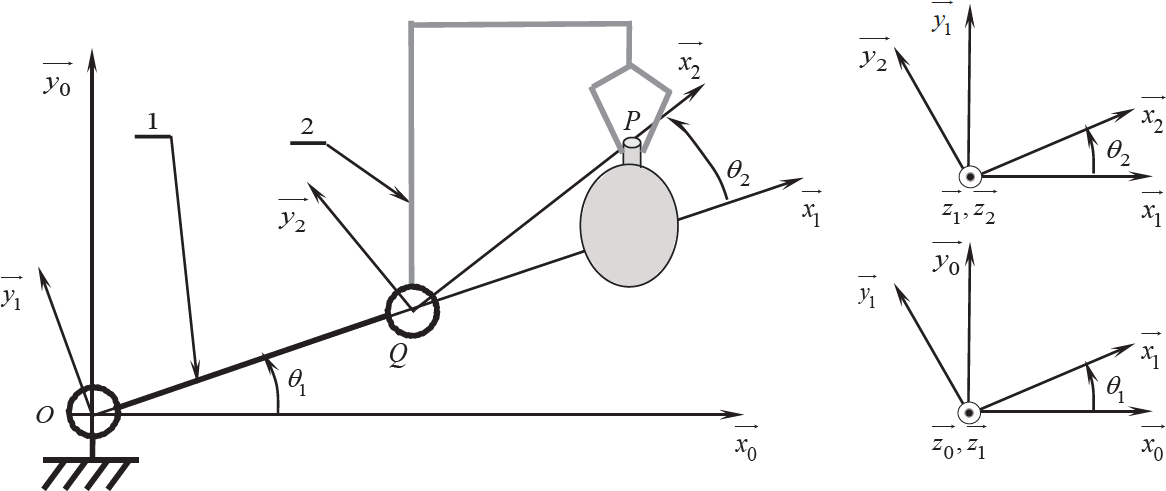
\includegraphics[width=.4\linewidth]{fig_07}
\caption{\label{fig_07} Consigne de vitesse}
\end{figure}

Lorsque le point focal de la tête optique suit le profil
moyen de la surface, l’angle $\theta$ varie au voisinage
de 0\degres. Nous montrerons %(partie V*** du sujet) 
que cette
variation de position est d’amplitude très faible, et
qu’en conséquence, il est possible de réaliser une linéarisation de ces équations au voisinage de 0\degres ( $\theta$ reste
petit). Nous supposons également que les termes de la forme $a\ddot{\theta}$  et $b\dot{\theta}^2$ sont négligeables devant le terme en $\ddot{x}$.
La loi de commande de l’unité de translation est représentée à la \autoref{fig_07}. La vitesse nominale (constante)
recherchée est notée ($V_0$). L’accélération maximale est notée ($A_{\text{cMax}}$).

\fi

\question{\label{q_07}En utilisant les simplifications mentionnées, déterminez, dans la phase d’accélération, puis dans la phase de déplacement à vitesse constante, les expressions littérales de $C_{\text{m1}}$ et $C_{\text{m3}}$.
Calculez la valeur du couple $C_{\text{m1}}$ maximal ($V_0 = \SI{0,2}{m.s^{-1}}$, $A_{\text{cMax}}=\SI{0,2}{m.s^{-2}}$).}
\ifprof
\begin{corrige}
En tenant compte des hyothèses : 
$ C_{\text{m3}} = B\ddot{\theta}  - m_3 r\theta \ddot{x} + f_3 \dot{\theta}   $

 $C_{\text{m1}} 
  =
   - \dot{x}\left( f_1\dfrac{2\pi}{\text{pas}} +f_2  \dfrac{\text{pas}}{2\pi}\right)
- \ddot{x}\left( \left( m_3+m_2 \right)\dfrac{\text{pas}}{2\pi}+ J_1 \dfrac{2\pi}{\text{pas}} \right)
$


Le couple maximal est atteint en fin d'accélération. Dans les conditions données, le temps d'accélération est donné par 
$V_0 = A_{\text{cMax}} t_a$ soit $ t_a  = \dfrac{A_{\text{cMax}}}{V_0} = \SI{1}{s}$.

On a donc 
 $C_{\text{m1 max}} 
  =
   - V_0\left( f_1\dfrac{2\pi}{\text{pas}} +f_2  \dfrac{\text{pas}}{2\pi}\right)
-  A_{\text{cMax}}\left( \left( m_3+m_2 \right)\dfrac{\text{pas}}{2\pi}+ J_1 \dfrac{2\pi}{\text{pas}} \right) = -\SI{0,128}{Nm}$.

\end{corrige}
\else
\fi

\ifprof
\else
Le choix des moteurs (M1 et M3) se fera à partir d’un cahier des charges, dont le couple maximal
transmissible par les moteurs est une des caractéristiques. Il existe bien d’autres spécifications comme, la
vitesse et l’accélération maximale, la surintensité supportée, l’encombrement axial et longitudinal…
\fi

\section{Commande de l'unité de rotation (UR)}
\ifprof
\else
Ce rugosimètre ne peut fonctionner, dans des conditions idéales, que si le point focal (P) de la tête optique
se situe en permanence au plus près du profil moyen de la pièce. Ceci nécessite, entre autres, un réglage
affiné des paramètres du correcteur de la chaîne d’asservissement associée à l’Unité de Rotation.

\begin{figure}[H]
\centering
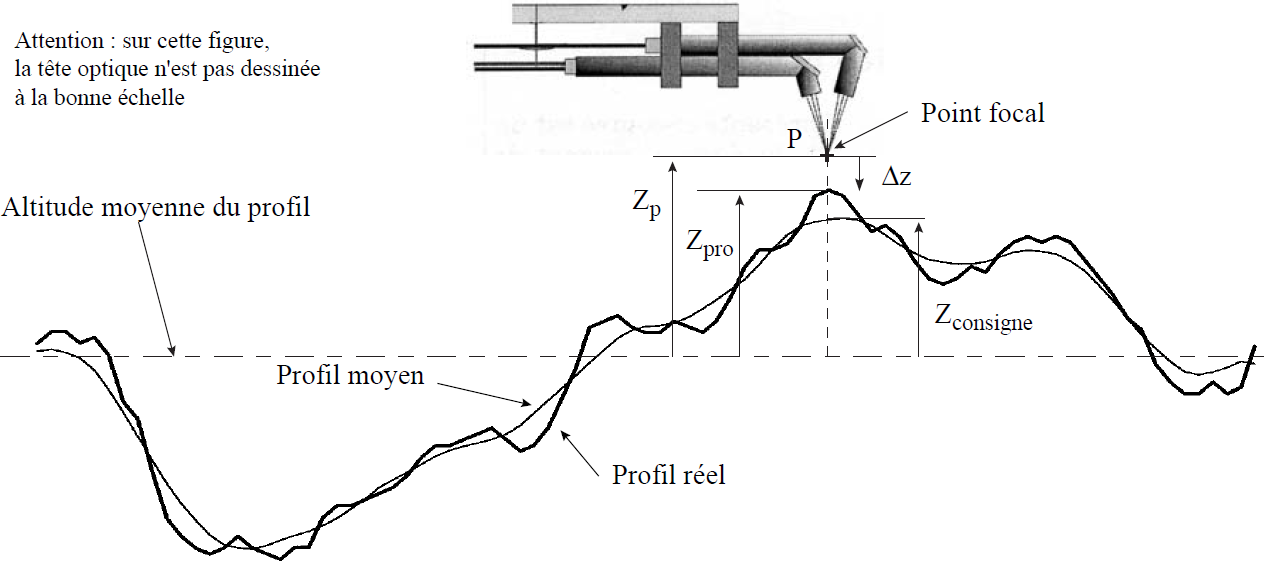
\includegraphics[width=.7\linewidth]{fig_08}
\caption{\label{fig_08} Profil réel / profil moyen et grandeurs utilisées}
\end{figure}

La \autoref{fig_08} illustre la problématique de mesure du profil de la pièce et met en place les différentes
grandeurs utilisées dans la chaîne d’asservissement de l’unité de rotation :
\begin{itemize}
\item la tête optique (capteur optique) permet de mesurer la distance entre le point focal (P) du système
optique et le profil réel de la pièce. Le signal de sortie de ce système est $\Delta z$ avec
$\Delta z(t)=z_{\text{pro}}(t)-z_p(t)$;
\item le pilotage (en altitude) du point focal (P) de la tête optique se fait sur une consigne particulière : la
position moyenne du profil de rugosité. Cette consigne $z_c$ est obtenue par une opération « Calcul de
la moyenne » qui détermine la moyenne mobile, sur un temps caractéristique $\tau$, de l’altitude du
profil de la pièce. La position réelle du point focal $z_p(t)$ est mesurée par l’intermédiaire d’un
capteur.
\end{itemize}
Avant de commencer une mesure, l’altitude moyenne de la pièce à mesurer est réglée (par un mécanisme,
non décrit dans cette étude), de telle façon qu’au début de la mesure le profil réel de la pièce soit
($z_{\text{pro}}(t=0)=0$), ce qui correspond à une consigne du bras $\theta_c$ également nulle : ($\theta_{c}(t=0)=0$).
Dans toute cette partie, vous considérerez que l’angle de rotation du bras (3) reste petit.
Le schéma bloc de l’unité de mesure est décrit à la \autoref{fig_09}.


\begin{figure}[H]
\centering
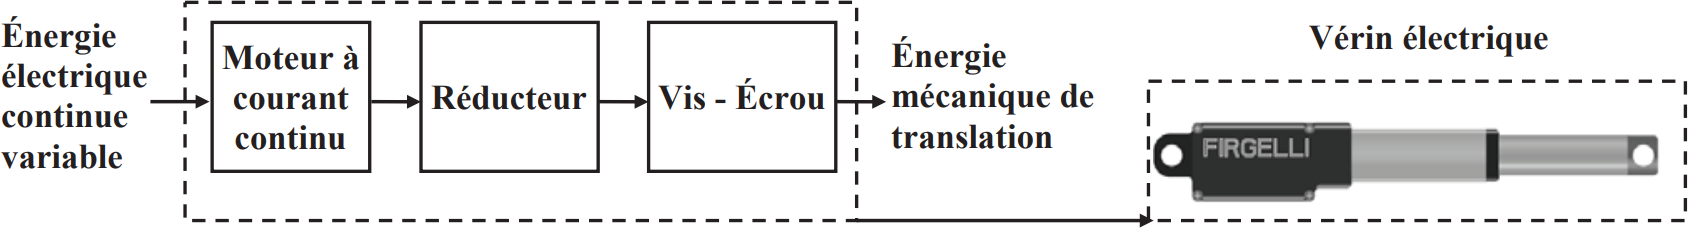
\includegraphics[width=.8\linewidth]{fig_09}
\caption{\label{fig_09} Schéma fonctionnel de l’unité de mesure}
\end{figure}

\begin{multicols}{2}
\begin{itemize}
\item $Z_{\text{pro}}$ : profil réel de la pièce (m);
\item $Z_{\text{mes}}$ : profil mesuré de la pièce (m);
\item $Z_{C}$ : consigne de position du point focal (m);
\item $\theta_{C}$ : consigne de position du bras (\si{rad});
\item $\theta$ : position du bras (3) (\si{rad});
\item $Z_{p}$ : position verticale du point focal (m);
\item $\Delta z$ : mesure réalisée par la tête optique (m);
\item $\text{Pert}$ : perturbation créée sur la position du bras (3), par l'accélération longitudinale (\si{Nm}).
\end{itemize}
\end{multicols}

Les fonctions de transfert associées aux différents éléments sont données ci-après : 
\begin{itemize}
\item tête optique : $H_{\text{opt}}(p)$;
\item adaptateur : $H_{\text{ada}}(p)=K_{\text{ada}}$ avec $K_{\text{ada}}=\SI{20}{rad.m^{-1}}$;
\item bras : $H_{\text{bras}}(p)=K_{\text{bras}}$ avec $K_{\text{bras}}=\SI{5e-2}{m.rad^{-1}}$;
\item calcul de la moyenne : $H_{\text{moy}}(p)$;
\item unité de rotation : $H_{\text{rot}}(p)$.
\end{itemize}

\fi


\subsection{Caractérisation globale de l'unité de mesure}

\ifprof
\else
Afin d’optimiser les performances du capteur de rugosité, l’exactitude de la mesure, la rapidité de la
mesure, la stabilité de l’ensemble…, il est nécessaire de déterminer la relation entre la fonction de transfert
globale et les fonctions de transfert élémentaires. Pour optimiser cette réponse globale, il sera possible de
modifier localement certains composants, puis de réinjecter dans le calcul complet les nouvelles fonctions
de transfert de ces composants.
\fi

\question{\label{q_08} En supposant que le système se déplace à vitesse constante (pas de perturbation), déterminez la fonction de transfert globale de l’unité de mesure : $F_{\text{G mes}}(p)=\dfrac{Z_{\text{mes}}(p)}{Z_{\text{pro}}(p)}$.}
\ifprof
\begin{corrige}
On note $G(p)=H_{\text{moy}}(p) K_{\text{ada}} H_{\text{rot}}(p) K_{\text{bras}}$.

On a alors $Z_{\text{mes}}(p)=\Delta_z(p)+Z_p = \left( Z_{\text{pro}}(p) -Z_p(p)\right)  H_{\text{opt}}(p)+Z_p(p)$.
De plus $Z_p (p)= Z_{\text{mes}}(p) G(p)$; donc 

$Z_{\text{mes}}(p)=  \left( Z_{\text{pro}}(p) - Z_{\text{mes}}(p) G(p)\right)  H_{\text{opt}}(p)+ Z_{\text{mes}}(p) G(p)$ 
$\Leftrightarrow Z_{\text{mes}}(p) \left(1+G(p) H_{\text{opt}}(p) - G(p) \right)=   Z_{\text{pro}}(p)  H_{\text{opt}}(p)$. 

Au final,  $F_{\text{G mes}}(p)=\dfrac{H_{\text{opt}}(p)}{1+G(p) H_{\text{opt}}(p) - G(p)} = 
\dfrac{H_{\text{opt}}(p)}{1+H_{\text{moy}}(p) K_{\text{ada}} H_{\text{rot}}(p) K_{\text{bras}}\left( H_{\text{opt}}(p) - 1\right)}$

\end{corrige}
\else
\fi

\subsection{Calcul de la moyenne mobile}
\ifprof
\else
Pour déterminer la consigne de position $z_c$ du point focal (P) de la tête optique, il est nécessaire de
calculer la position moyenne du profil. Plusieurs techniques peuvent être utilisées, l’une des plus simples
est de définir cette consigne comme étant la moyenne, sur un temps donné, des positions antérieures. Ceci
s’écrit mathématiquement : $z_c(t)=\dfrac{\int\limits_{t-\tau}^{t}z_{\text{mes}}(v)\dd v}{\tau}$.
\fi




\question{\label{q_}Montrez que la transmittance $H_{\text{moy}}(p)$ peut se mettre sous la forme :
$H_{\text{moy}}(p) = \dfrac{Z_c(p)}{Z_{\text{mes}}(p)}=\dfrac{1-\text{e}^{-p\tau}}{p \tau}$.}
\ifprof
\begin{corrige}
On a $z_c(t)=\dfrac{1}{\tau} \int\limits_{t-\tau}^{t}z_{\text{mes}}(v)\dd v$ 
$=\dfrac{1}{\tau} \left( \int\limits_{0}^{t}z_{\text{mes}}(v)\dd v - \int\limits_{0}^{t-\tau}z_{\text{mes}}(v)\dd v \right)$. En passant dans le domaine de Laplace en utilisant le théorème de l'intégration et du retard, on a : 
$Z_c(p)=\dfrac{1}{\tau} \left( \dfrac{1}{p}Z_{\text{mes}}(p)- \dfrac{1}{p}Z_{\text{mes}}(p)\text{e}^{-\tau p}  \right)$$=\dfrac{1}{\tau p} Z_{\text{mes}}(p)\left( 1- \text{e}^{-\tau p}  \right)$.

On a donc $H_{\text{moy}}(p) = \dfrac{Z_c(p)}{Z_{\text{mes}}(p)}=\dfrac{1-\text{e}^{-p\tau}}{p \tau}$.

\end{corrige}
\else
\fi

\subsection{Etude détaillée de l'unité de rotation}

\ifprof
\else

La seule fonction qu’il reste à caractériser, puis à optimiser, est celle de l’Unité de Rotation (Moteur
couple + Tête optique). Le schéma bloc de ce système est donné à la \autoref{fig_10}.


\begin{figure}[H]
\centering
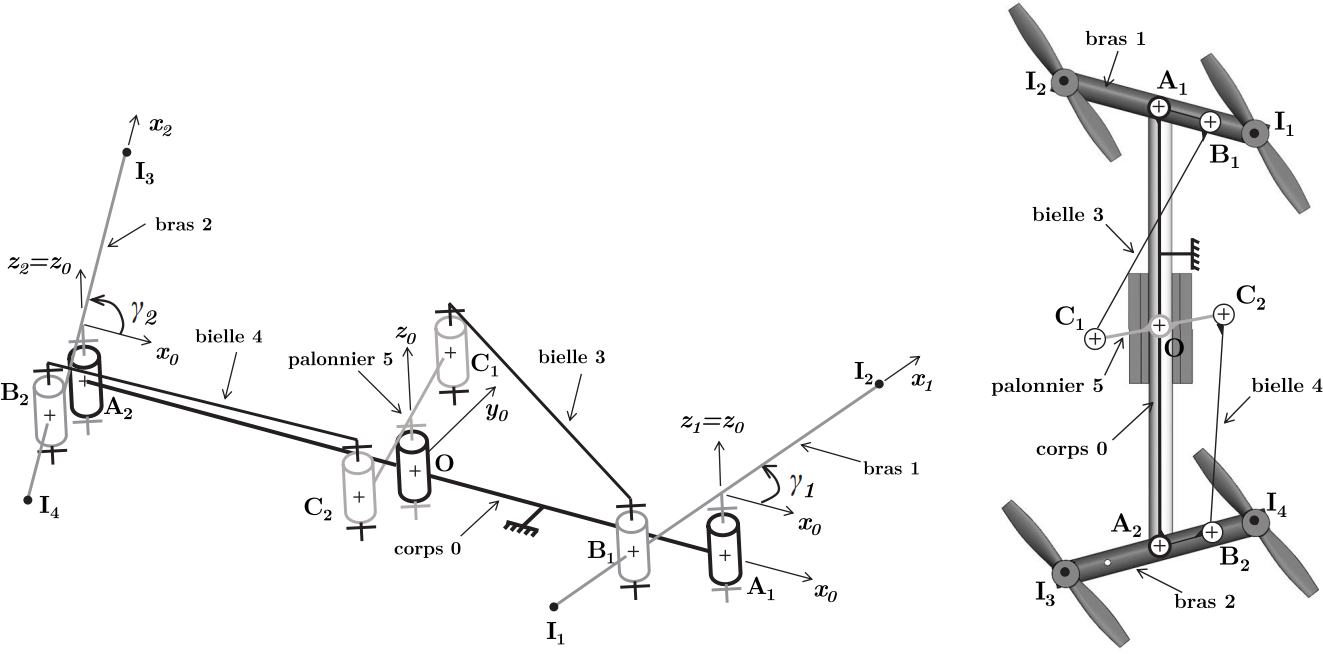
\includegraphics[width=.7\linewidth]{fig_10}
\caption{\label{fig_10} Schéma-blocs de la commande du moteur couple}
\end{figure}


\begin{multicols}{2}
\begin{itemize}
\item $\theta_c$ consigne de position du bras (rad);
\item $I_{\theta}$ intensité correspondant à la consigne (A);
\item $I_{\text{capt}}$ intensité en sortie du capteur angulaire (A);
\item $I_{\text{mot}}$ intensité d’alimentation du moteur couple (A);
\item $C_{\text{m3}}$ couple moteur développé (Nm);
\item $C_{\text{pert acc}}$ couple perturbateur créé lors de l’accélération de
l’unité de translation (Nm);
\item $\theta$ position angulaire du bras (3) (rad).
\end{itemize}
\end{multicols}

Les fonctions de transfert associées aux différents éléments sont données ci-après :
\begin{multicols}{2}
\begin{itemize}
\item convertisseur : $H_{\text{con}}(p)=K_{\text{con}}$, avec $K_{\text{con}}=\SI{2}{A.rad^{-1}}$;
\item moteur : $H_{\text{mot}}(p)=K_{\text{mot}}$, avec $K_{\text{mot}}=\SI{0,05}{N.m.A^{-1}}$;
\item tête optique et système de rappel : $$H_{\text{tête}}(p)=\dfrac{K_t}{1+\dfrac{2\xi}{\omega_0}p+\dfrac{p^2}{\omega_0^2}};$$
\item capteur : $H_{\text{capt}}(p)=K_{\text{capt}}=K_{\text{con}}$;
\item correcteur : $H_{\text{Cor}}(p)$.
\end{itemize}
\end{multicols}
\fi

\subsubsection{Identification des paramètres de la tête optique}

\ifprof
\else

Pour identifier les paramètres du modèle associé à la tête optique, on soumet le système, décrit à la \autoref{fig_11}, à un échelon d’intensité d’amplitude (\SI{2,5}{mA}). La
réponse indicielle de ce système est donnée à la \autoref{fig_12}. La réponse a été adimensionnée (position / position
finale) pour faciliter les calculs ultérieurs. La valeur asymptotique finale est : \SI{158e-6}{rad}.


\begin{figure}[H]
\centering
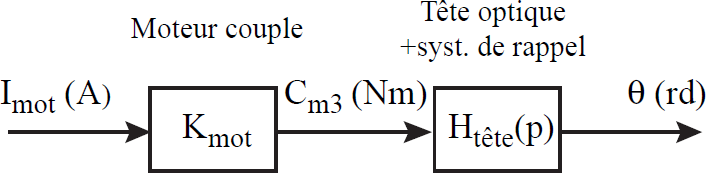
\includegraphics[width=.4\linewidth]{fig_11}
\caption{\label{fig_11} Système testé en réponse indicielle}
\end{figure}


\begin{figure}[H]
\centering
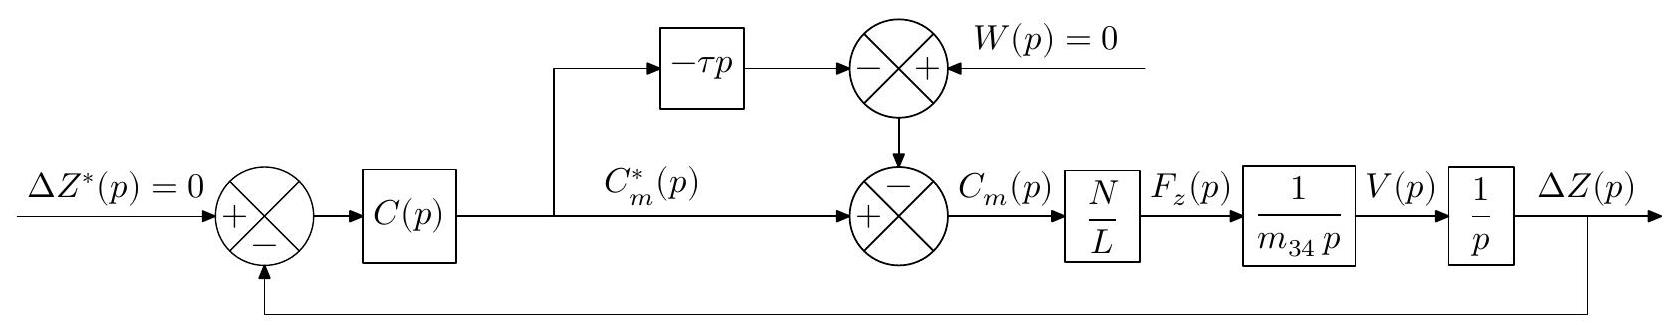
\includegraphics[width=.6\linewidth]{fig_12}
\caption{\label{fig_12} Réponse indicielle adimensionnée (sortie/valeur finale de la sortie)}
\end{figure}
\fi


\question{\label{q_10}En utilisant la réponse indicielle de la \autoref{fig_12}, justifiez et critiquez le modèle qui a été retenu pour décrire, d’un point de vue mécanique, la fonction de transfert de la tête optique et du système de rappel :
$H_{\text{tête}}(p)=\dfrac{K_t}{1+\dfrac{2\xi p}{\omega_0}+\dfrac{p^2}{\omega_0^2}}$. Vous analyserez très finement les différents dépassements. Donnez, après identification, les valeurs numériques et les unités des paramètres ($K_t$, $\xi$, $\omega_0$).
Expliquez clairement votre démarche d’identification. Vous pouvez utiliser les abaques des figures
\autoref{fig_13} et \autoref{fig_14}. Toutes les grandeurs mesurées sur les figures \autoref{fig_12}, \autoref{fig_13} et \autoref{fig_14} devront être mentionnées sur les
figures du document réponse.}
\ifprof
\begin{corrige}
La tangente nulle à l'origine et les multiples dépassements peuvent indiquer que le comportement du système est celui d'un ordre 2 avec $\xi<0,7$.

Ici le premier dépassement est de 30\,\% et le second dépassement est de 40\,\%. cet accroissement du dépassement indique qu'un ordre 2 ne sera qu'un modèle approché. 

En utilisant les abaques, un premier dépassement de 30\,\% permet de choisir un coefficient d'amortissement $\xi =0,35$. 

La pseudo période est de l'ordre de \SI{0,023}{s} soit une pulsation approximativement de \SI{290}{rad.s^{-1}}.

Enfin, le gain est donné  par $ \dfrac{ \SI{158e-6}{rad}}{\SI{2,5e-3}{A}}=K_{\text{mot}} K_t $ soit 
$  K_t = \dfrac{ \SI{158e-6}{rad}}{\SI{2,5e-3}{A}\SI{0,05}{NmA^{-1}}}= \dfrac{ \SI{158e-6}{rad}}{\num{2,5e-3}\times \SI{0,05}{Nm}} =\SI{1,2}{rad.Nm^{-1}}$.
\end{corrige}
\else
\fi


\ifprof
\else
\begin{minipage}[c]{.47\linewidth}
\begin{figure}[H]
\centering
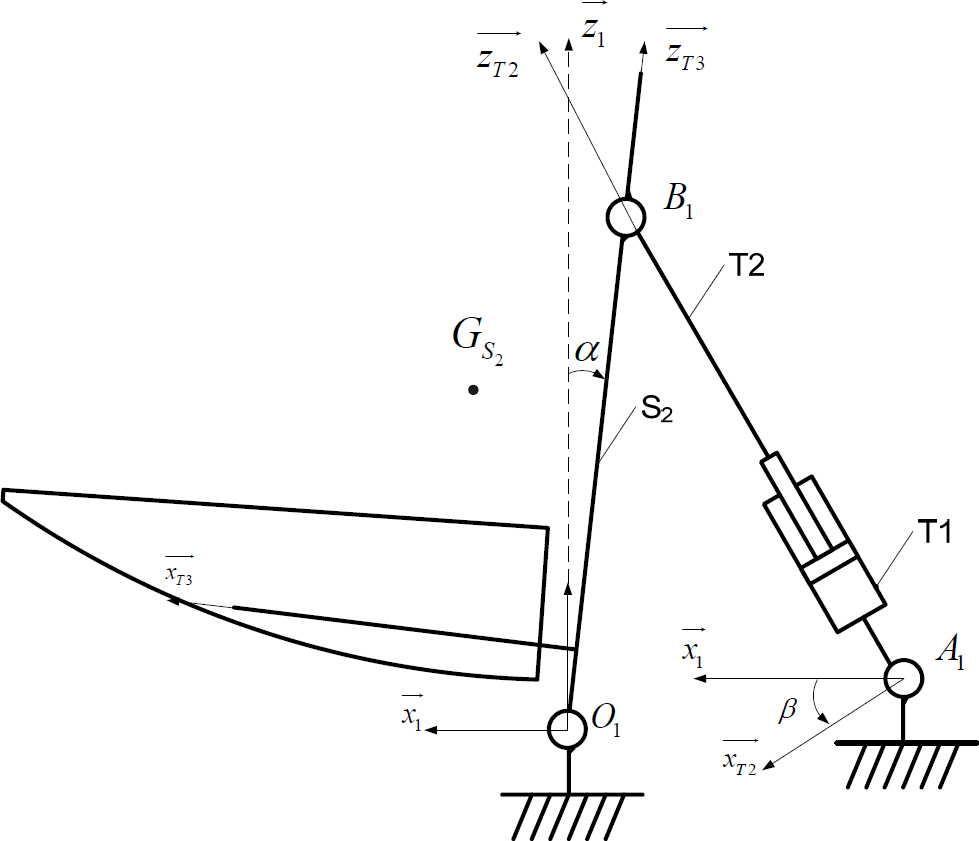
\includegraphics[height=5cm]{fig_13}
\caption{\label{fig_13} Dépassement relatif (\%) (1 = 100~\%) en fonction
du coefficient d’amortissement et du numéro du dépassement}
\end{figure}
\end{minipage}\hfill
\begin{minipage}[c]{.47\linewidth}
\begin{figure}[H]
\centering
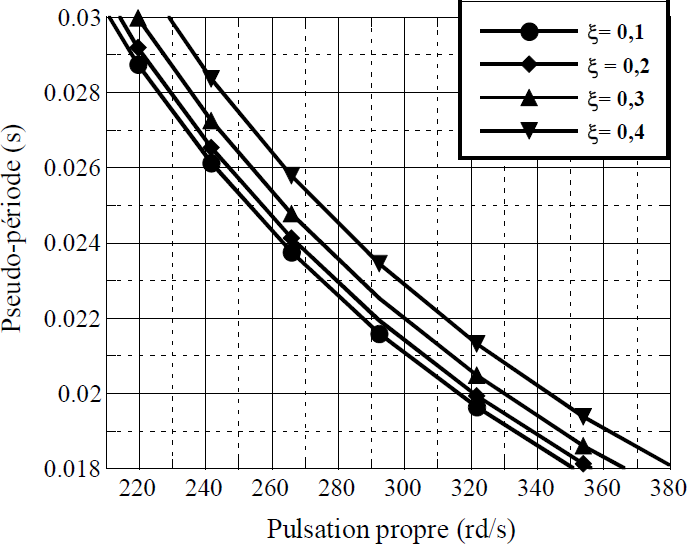
\includegraphics[height=5cm]{fig_14}
\caption{\label{fig_14} Pseudo période en fonction de la pulsation
propre et du coefficient d’amortissement}
\end{figure}
\end{minipage}

\vspace{.25cm}

Une identification, plus fine (à l’aide de moyens informatiques), a permis de déterminer les valeurs des
paramètres de $H_{\text{tête}}(p)$. Quels que soient les résultats que vous avez trouvés à la question \ref{q_10}, et sans
présager de la corrélation de ces valeurs numériques et des vôtres, vous prendrez pour la suite du
problème : $K_t =\SI{1,2}{U.S.I.}$, $\xi = 0,2$ , $\omega_0 = \SI{300}{U.S.I.}$.


Ces paramètres permettent de remonter aux caractéristiques matérielles, inertielles, des pièces ainsi qu’aux
caractéristiques dissipatives des liaisons non parfaites. Dans cet essai, il n’y a pas de translation de
l’ensemble du rugosimètre.
\fi



\question{\label{q_11}Donnez les relations liant les paramètres de la fonction de transfert 
$H_{\text{tête}}(p)$ et ceux utilisés à la question~\ref{q_04} (calcul de ($C_{\text{m3}}$), qui est maintenant noté
($C_{\text{m}}$), lorsque l’accélération est nulle et lorsque l’on reste au voisinage de ($\theta=0\degres$)).
Donnez les valeurs numériques des coefficients $K_{\text{tors}}$ (raideur du ressort torsion), $f_3$ (coefficient de
frottement visqueux) et $B$ (moment d’inertie). }
\ifprof
\begin{corrige}
En reprenant l'équation précédente, on a $ C_{\text{m3}} = B\ddot{\theta}  + K_{\text{tor}}\theta+ f_3 \dot{\theta}   $.
En passant dans le domaine de Laplace, on a $H_{\text{tête}}(p) = \dfrac{\theta(p)}{C_{\text{m3}}(p)} = \dfrac{1}{Bp^2+f_3p+K_{\text{tor}}}$ $= \dfrac{\dfrac{1}{K_{\text{tor}}}}{\dfrac{B}{K_{\text{tor}}}p^2+\dfrac{f_3}{K_{\text{tor}}}p+1}$.

On a donc $\dfrac{1}{K_{\text{tor}}} = K_t$ soit $K_{\text{tor}}=\dfrac{1}{K_t} = \SI{0,83}{Nm.rad^{-1}}$. 

$\dfrac{2\xi}{\omega_0} = \dfrac{f_3}{K_{\text{tor}}}$ soit $f_3 = \dfrac{2\xi K_{\text{tor}} }{\omega_0} = \SI{1e-3}{Nms.rad^{-1}}$

$\dfrac{1}{\omega_0^2} = \dfrac{B}{K_{\text{tor}}}$ soit $B=\dfrac{K_{\text{tor}}}{\omega_0^2 } = \SI{9,3e-6}{kg.m^2}$
\end{corrige}
\else
\fi

\subsubsection{Choix du correcteur}

\ifprof
\else
Afin de suivre, de la façon la plus fine possible, le profil moyen de la pièce, il est nécessaire de choisir
avec soin le correcteur afin d’assurer la précision, la rapidité et la stabilité de la position du point focal (P)
donc la position du bras~(3).

En ce qui concerne la précision de position angulaire du bras, les concepteurs de ce rugosimètre
souhaitent :
\begin{itemize}
\item annuler, en régime permanent, l’influence d’une perturbation de type échelon. Cette forme de
perturbation peut être rencontrée lors de la phase d’accélération de l’unité de translation;
\item limiter au maximum, sans nécessairement l’annuler, l’erreur de positionnement pour une consigne
de type rampe (erreur de traînage). Cette entrée est suffisamment représentative si l’on considère un
profil moyen qui serait décrit par la figure \ref{fig_15}.
\end{itemize}
\begin{figure}[H]
\centering
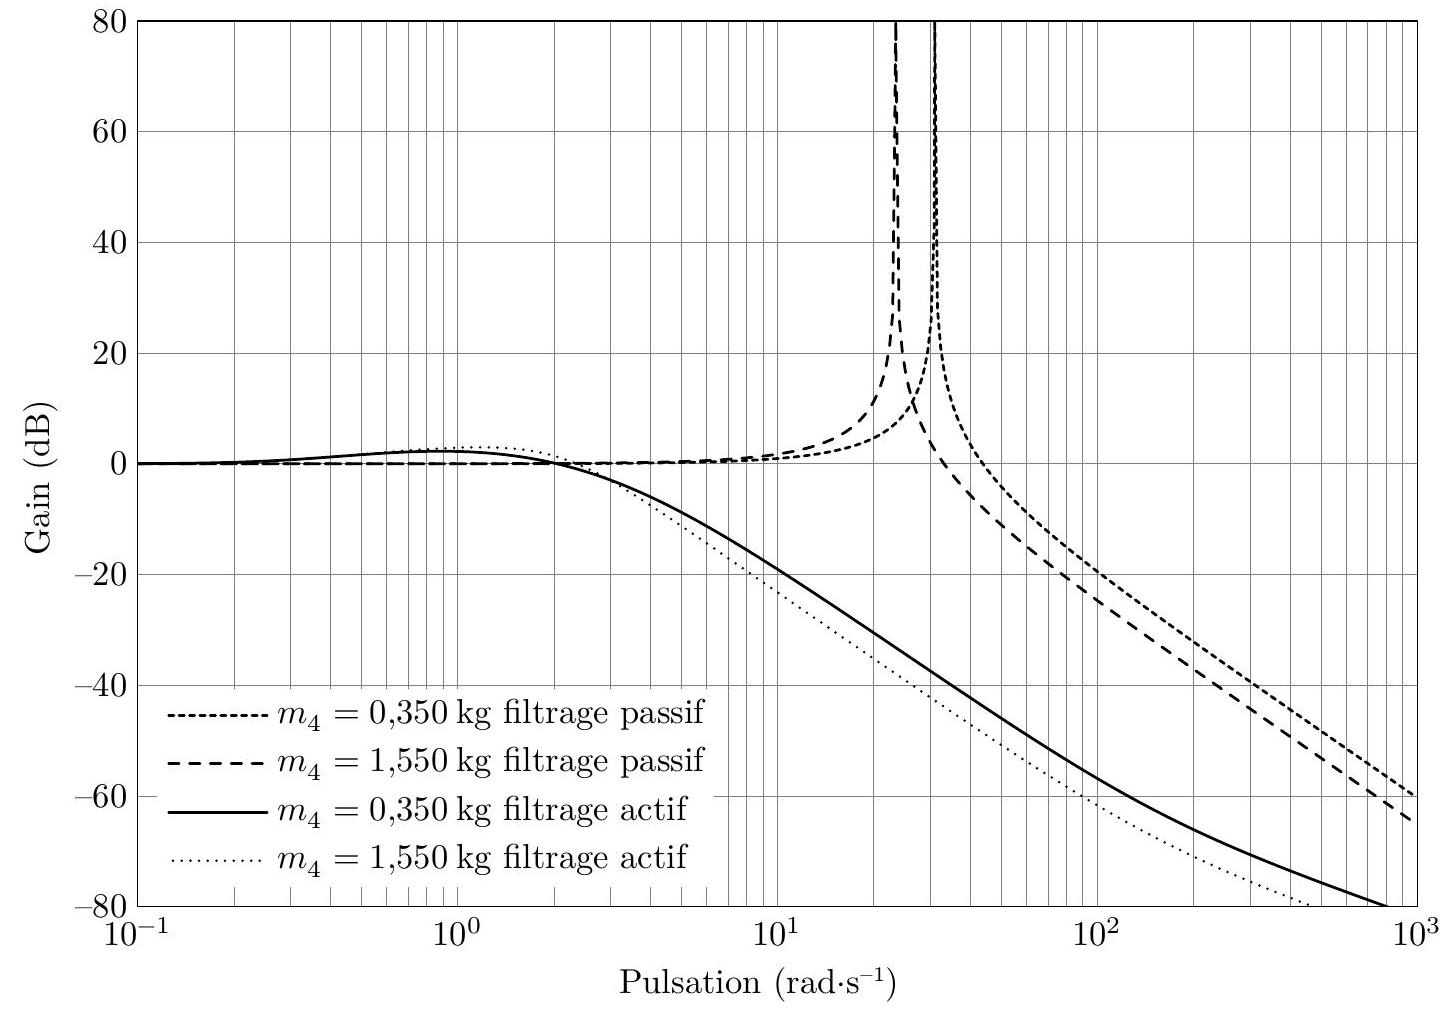
\includegraphics[width=.7\linewidth]{fig_15}
\caption{\label{fig_15} Description du profil par plusieurs fonction rampes}
\end{figure}

Pour cette exigence du cahier des charges, les concepteurs envisagent trois choix possibles : un correcteur
proportionnel, un correcteur proportionnel-intégral, et un correcteur dont la fonction de transfert est
$H_{\text{cor}}(p) = \dfrac{K_p}{p^2}$.

\fi

\question{\label{q_12}Donnez, parmi ces trois choix, le ou les correcteurs qui respecte(nt) les critères de précision.
Quelles sont les conséquences sur la stabilité de ces correcteurs ?
Quel est votre choix final (justifiez votre réponse).
Vos réponses devront être clairement argumentées (résultats de cours ou démonstrations).}
\ifprof
\begin{corrige} ~\\

La FTBO du système est donné par $\text{FTBO}(p)=H_{\text{cor}}(p)K_{\text{mot}}H_{\text{tete}}(p)$ avec 
$H_{\text{tete}}(p)$ une fonction d'ordre 2 et de classe 0. 

\begin{center}
\begin{tabular}{cccc}
\hline
& Correcteur P & Correcteur PI & Correcteur << II >> \\\hline
& $C(p)=K_P$    & $C(p)=K_P + \dfrac{K_I}{p}$ & $C(p)= \dfrac{K_p}{p^2}$  \\  \hline
Classe de la BO & 0 & 1 & 2 \\\hline
Stabilité  & Oui & ??? & Non \\\hline
Ecart statique & $\dfrac{1}{1+K_PK_tK_{\text{mot}}}$ & 0 & (0)\\\hline
Ecart de trainage & $\infty$ & $\dfrac{1}{K_PK_tK_{\text{mot}}/K_I}$ & (0)\\\hline
\end{tabular}
\end{center}
Le choix se tourne vers le correcteur proportionnel intégral en réglant les paramètres permettant de garantir la stabilité et l'erreur de trainage souhaitée. 
\end{corrige}
\else
\fi


Pour diverses raisons, que nous n’exposerons pas dans le sujet, le choix des concepteurs s’est finalement
porté sur un correcteur dont la fonction de transfert est 
$H_{\text{cor}}(p) = \dfrac{K_p}{p}$ et dont il reste à déterminer le
coefficient ($K_p$).


Le cahier des charges de l’unité de rotation nous impose d’avoir des marges de stabilité suffisantes, tout en
ayant un système qui soit le plus rapide possible. La marge de phase doit être d’au moins 45\degres et la marge
de gain minimale est de \SI{6}{dB}.

\question{\label{q_13}Déterminez (en justifiant votre réponse, votre démarche) le gain ($K_p$) optimal, vis-à-vis des marges de stabilité, du correcteur. Vous pouvez utiliser et compléter, si vous le jugez nécessaire, les diagrammes du document réponse (graphe semi-logarithmique).}
\ifprof
\begin{corrige}
On a $\text{FTBO}(p)=\dfrac{0,12}{1+\dfrac{2\times 0,2}{300}p+\dfrac{p^2}{300^2}} \dfrac{K_p}{p}$.

\begin{center}
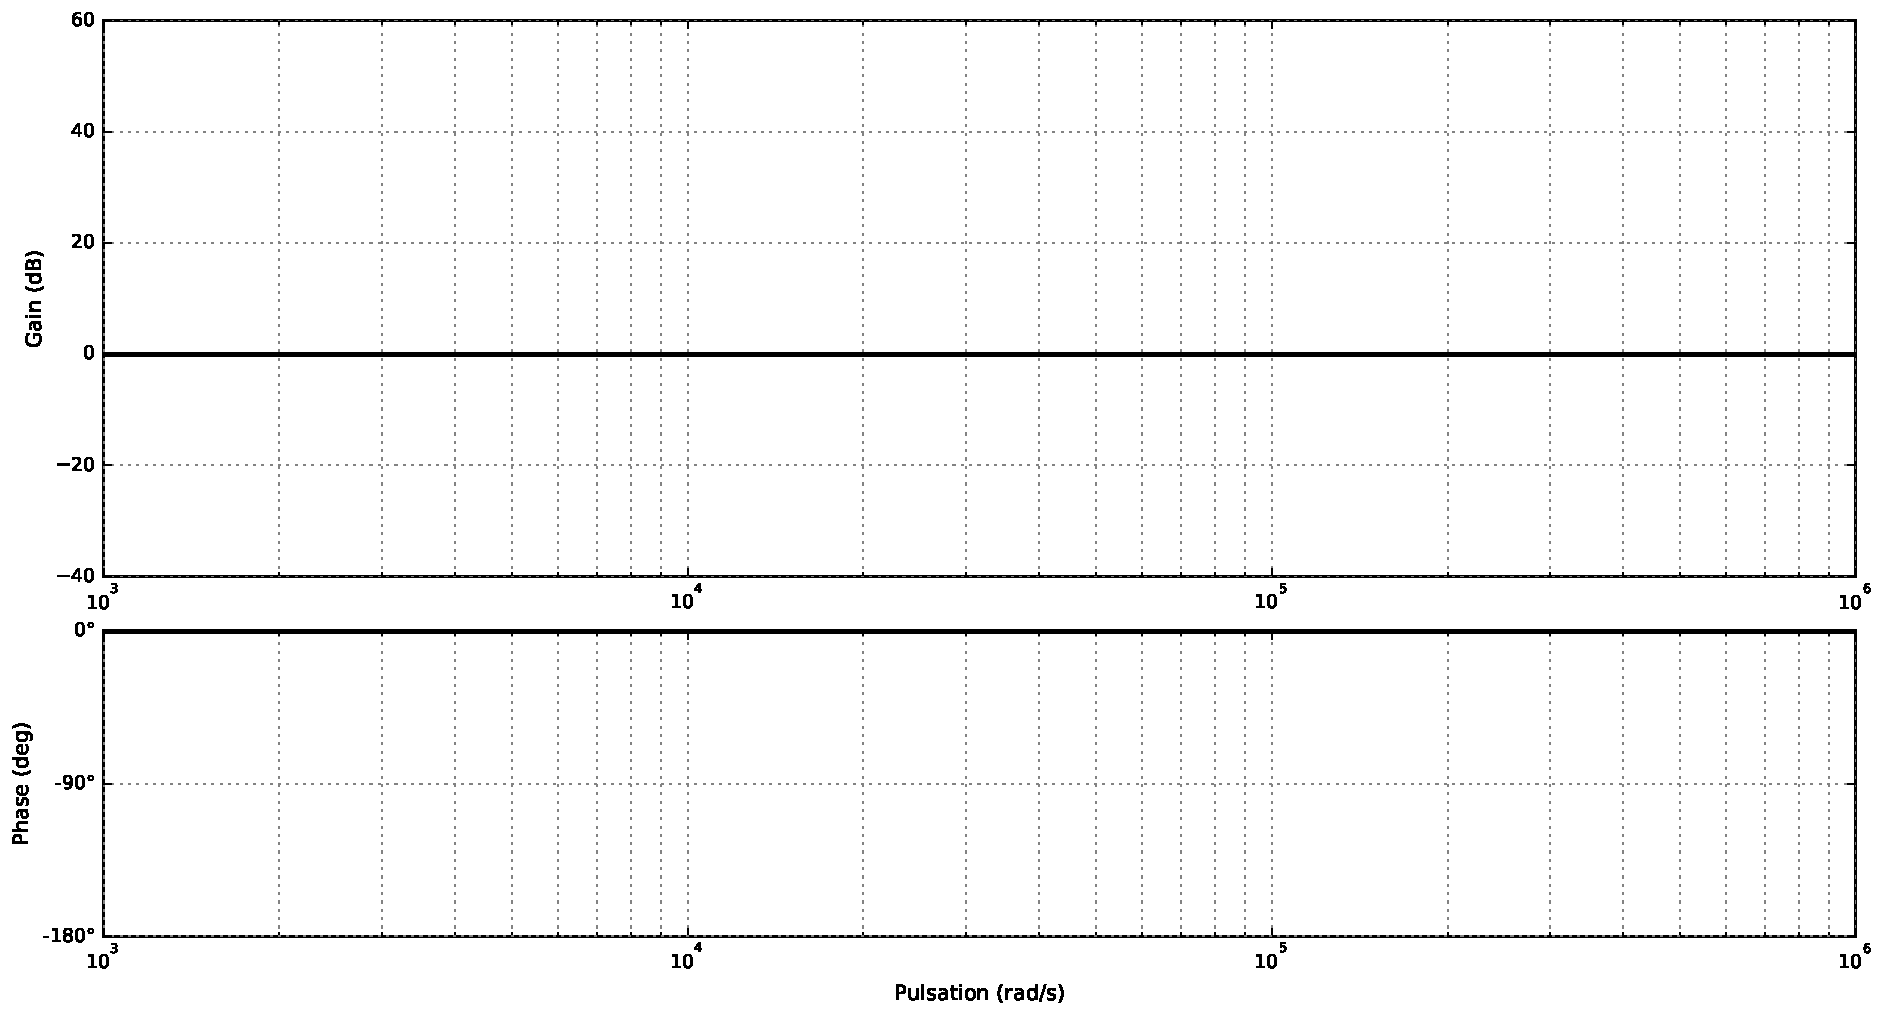
\includegraphics[width=.8\linewidth]{cor_02}
\end{center}

Le système est stable. 

Pour avoir une marge de phase de 45\degres, il faut remonter le gain de \SI{60}{dB} soit $K_p = 1000$.

De mêle pour avoir une marge de gain de \SI{6}{dB}, il faut remonter le gain de \SI{54}{dB}.
\end{corrige}
\else
\fi

\ifprof
\else

À toute fin utile, le tableau ci-dessous donne les phases (en \degres) et les modules (en dB) de la
transmittance  $H(j\omega )=\dfrac{1}{1+\dfrac{0,4 }{300}j\omega-\dfrac{1}{9\times 10^4}\omega^2}$
différentes valeurs de pulsations.

\begin{center}
\begin{tabular}{ccc}
\hline
Pulsation (rd/s) & Phase (\degres) & Amplitude (dB)  \\ \hline \hline
100 & -8,5 & 0,9 \\\hline
200 & -25,6 & 4,2\\ \hline
246 & -45,0 & 6,7\\ \hline
300 & -90,0 & 8,0\\ \hline
366 & -135,0 & 3,21\\ \hline
1000 & -172,5 & -20,2\\ \hline
\end{tabular}
\end{center}


%\question{\label{q_13a}Tracer le diagramme de la fonction de transfert en boucle ouverte $H_{\text{BO}}(p)=\dfrac{Kp}{p}K_{\text{mot}}\dfrac{K_t}{1+\dfrac{2\xi}{\omega_0}p+\dfrac{p^2}{\omega_0^2}}$.}
%
%\question{\label{q_13b}Déterminez (en justifiant votre réponse, votre démarche) le gain ($K_p$) optimal, vis-à-vis de la marge de gain, du correcteur. }
%
%\question{\label{q_13c}Déterminez (en justifiant votre réponse, votre démarche) le gain ($K_p$) optimal, vis-à-vis de la marge de phase, du correcteur.}
%
%\question{\label{q_13d}Conclure.}


Le réglage qui vient d’être réalisé concerne principalement la stabilité du système. La précision a été respectée
par le choix du type de correcteur (question \ref{q_12}). Il reste maintenant à se
pencher sur la rapidité de ce système.
Pour cela, nous avons simulé, avec un
logiciel dédié, la réponse indicielle du
système de commande de l’Unité de
Rotation (\autoref{fig_10}) pour trois valeurs de
($K_p$ ) : celle qui correspond au réglage des marges de stabilité
($K_{\text{p Marge stabilité}}$ ) , 90 \% de cette valeur
de $K_{\text{p Marge stabilité}}$ et 110 \% de
$K_{\text{p Marge stabilité}}$.

\begin{minipage}[c]{.47\linewidth}
\begin{figure}[H]
\centering
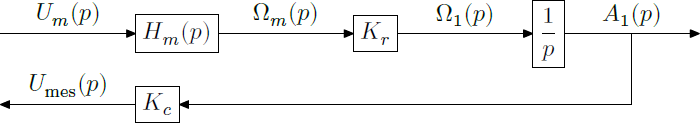
\includegraphics[height=4.5cm]{fig_16}
\caption{\label{fig_16}Réponse indicielle adimensionnée de l’Unité de Rotation}
\end{figure}
\end{minipage}\hfill
\begin{minipage}[c]{.47\linewidth}
\begin{figure}[H]
\centering
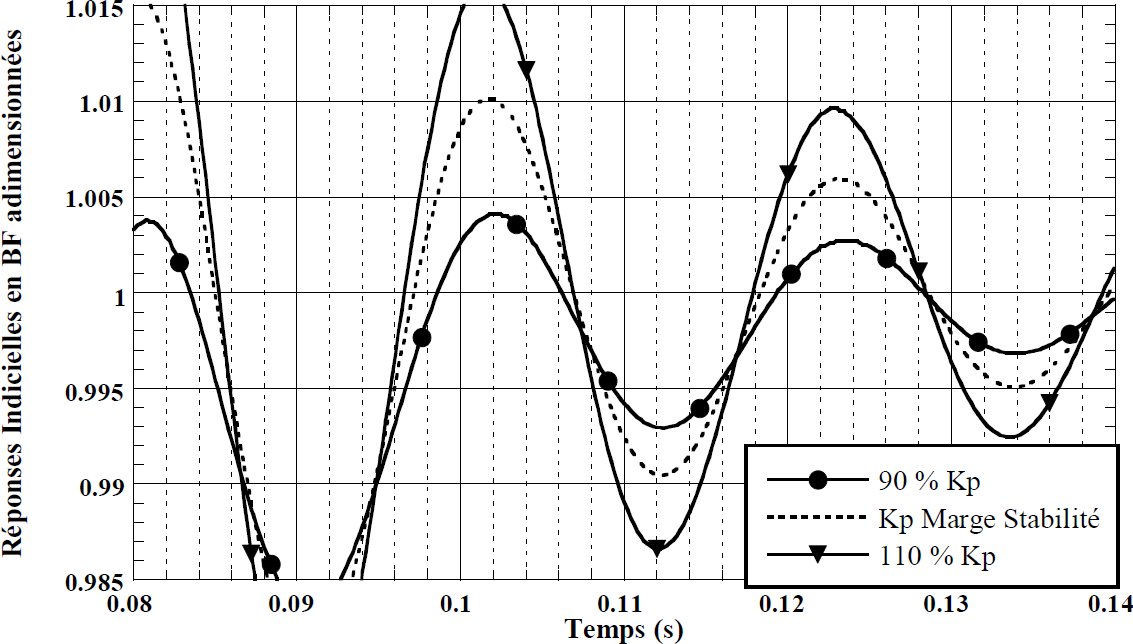
\includegraphics[height=4.5cm]{fig_16_bis}
\caption{\label{fig_16b} Zoom de la réponse indicielle adimensionnée de l’Unité de Rotation}
\end{figure}
\end{minipage}
\fi

\question{\label{q_14}Déterminer parmi ces trois courbes, celle qui présente le meilleur temps de réponse à \SI{1}{\%}. Donnez ce temps de réponse à \SI{1}{\%}. Réalisez les tracés nécessaires sur le document réponse.
Expliciter votre choix final du coefficient $K_p$ et conclure sur la commande de l’unité de rotation.}
\ifprof
\begin{corrige} ~\\
\begin{center}
\begin{tabular}{lcc}
\hline
$90\% K_p$ & \SI{0,095}{s} & \\ \hline
$K_p$ marge stab. &  \SI{0,103}{s}& \\ \hline
$110\% K_p$ & \SI{0,115}{s} & \\ \hline
\end{tabular}
\end{center}

Choix, rien ne semble empêcher de prendre le gain correspondant au respect des marges....
\end{corrige}
\else
\fi


\section{Amélioration de l’unité de positionnement en $Z$}
\ifprof
\else
Dans ce prototype, le positionnement vertical (en $z$) du point focal est obtenu par l’unité de rotation. Ceci a
plusieurs conséquences négatives sur le fonctionnement global du capteur :
\begin{itemize}
\item modification de la position longitudinale du point de mesure. Lorsque la tête optique tourne, la
mesure de ($z$) n’est pas réalisée à l’endroit désiré, ce qui induit une erreur dans la reconstruction de
la surface ;
\item modification de l’angle d’incidence des faisceaux optiques ;
\item modification de la position de la tête optique lors des phases d’accélération et de freinage de l’unité
de translation longitudinale (étudiée à la partie \ref{sec:3}).
\end{itemize}
\fi


\subsection{Étude de la position réelle longitudinale du point focal}
\ifprof
\else
Il vous est demandé, dans un premier temps, de quantifier l’écart de position
longitudinale obtenu lorsque l’on utilise la totalité du débattement vertical.
La \autoref{fig_17} illustre le problème d’erreur de positionnement longitudinal ($\Delta x$) créée
par la rotation de la tête de mesure. 
\begin{figure}[H]
\centering
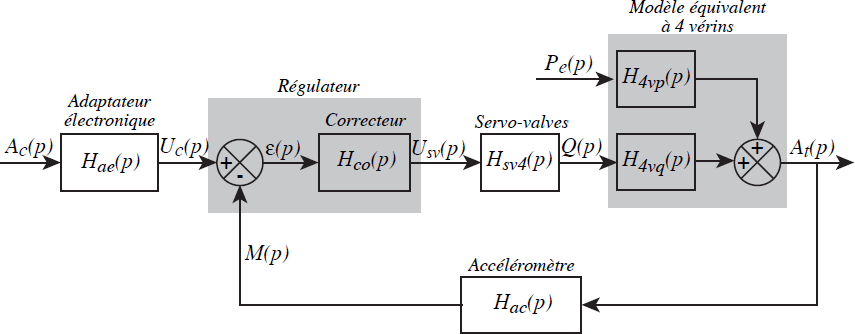
\includegraphics[width=.7\linewidth]{fig_17}
\caption{\label{fig_17} Incidence sur le positionnement du point focal lors de la rotation,de la tête optique}
\end{figure}

Données : 
$ \vect{AP} = a\vect{x_3}-b\vect{z_3}$ (avec $a = \SI{50}{mm}$ et $b =\SI{15}{mm}$);
$\Delta x = x_P(\theta)-x_P(0)$; $\Delta z = z_P(\theta) - z_P(0)$.

Le cahier des charges de ce système impose une variation verticale ($z$) du point
focal de $\pm \SI{5}{mm}$ par rapport à la position de référence ( $\theta = 0\degres$).

\fi

\question{\label{q_15}
Après avoir donné les expressions littérales des variations de position longitudinale ($\Delta x = f(\theta, a, b)$)
et verticale ($\Delta z = g(\theta, a, b)$) du point focal en fonction de la rotation de la tête optique, linéarisez ces
expressions afin d’obtenir une formule approchée donnant le rapport ($\Delta x / \Delta z$) : $\Delta x / \Delta z = h(a, b)$.
Donner la valeur numérique du décalage longitudinal maximal.
Conclure quant à la réalité du problème soulevé précédemment : « modification de la position
longitudinale du point de mesure ».}
\ifprof
\begin{corrige}
On a $\vect{AP} = a\vect{x_3}-b\vect{z_3}$. On projette cette relation dans la base $\rep{0}$ : 
 $\vect{AP} = a\left(\cos\theta \vect{x_0} - \sin\theta \vect{z_0}  \right) -b\left(\cos\theta \vect{z_0} + \sin\theta \vect{x_0}  \right)$.
 
 Par suite, 
 $\vect{AP_0} = a\vect{x_0}  -b\vect{z_0} $ et 
  $\vect{AP_{\theta}} = a\left(\cos\theta \vect{x_0} - \sin\theta \vect{z_0}  \right) -b\left(\cos\theta \vect{z_0} + \sin\theta \vect{x_0}  \right)$.

On a donc 
$\Delta x =  \left| a - \left(a\cos\theta   -b \sin\theta \right)\right|$ $=  \left| a - a\cos\theta +b \sin\theta \right| \simeq b\theta$ et

$\Delta z =  \left| -b - \left(-a\sin\theta -b\cos\theta \right)\right|$ $=  \left| -b +a\sin\theta +b\cos\theta \right|\simeq a\theta$.

Par suite, $\dfrac{\Delta x}{\Delta z} = \dfrac{b}{a}$. Ainsi, $\Delta_x = \dfrac{b}{a} \Delta z = \dfrac{15\times 5}{50}=\SI{1,5}{mm}$.

Conclusion ???
\end{corrige}
\else
\fi

\ifprof
\else
En plus de ce problème de position longitudinale du point focal, il y a aussi une modification de l’angle
d’incidence et de réflexion des faisceaux optiques par rapport à la surface de la pièce qui correspond à une
variation de ($2\theta$).
\fi

\subsection{Modification de l'unité de positionnement vertical du point focal}

\ifprof
\else
Afin de découpler les mouvements verticaux et longitudinaux du point focal lors des phases d’accélération
et de freinage de l’axe longitudinal (x), et d’éviter la rotation de la tête optique, les concepteurs de ce
capteur ont imaginé une autre chaîne cinématique pour le positionnement vertical du point focal.

Les principales caractéristiques du moteur couple donnant satisfaction, les concepteurs désirent conserver ce
système de motorisation. La \autoref{fig_18} représente le schéma cinématique plan du mécanisme envisagé.

\begin{figure}[H]
\centering
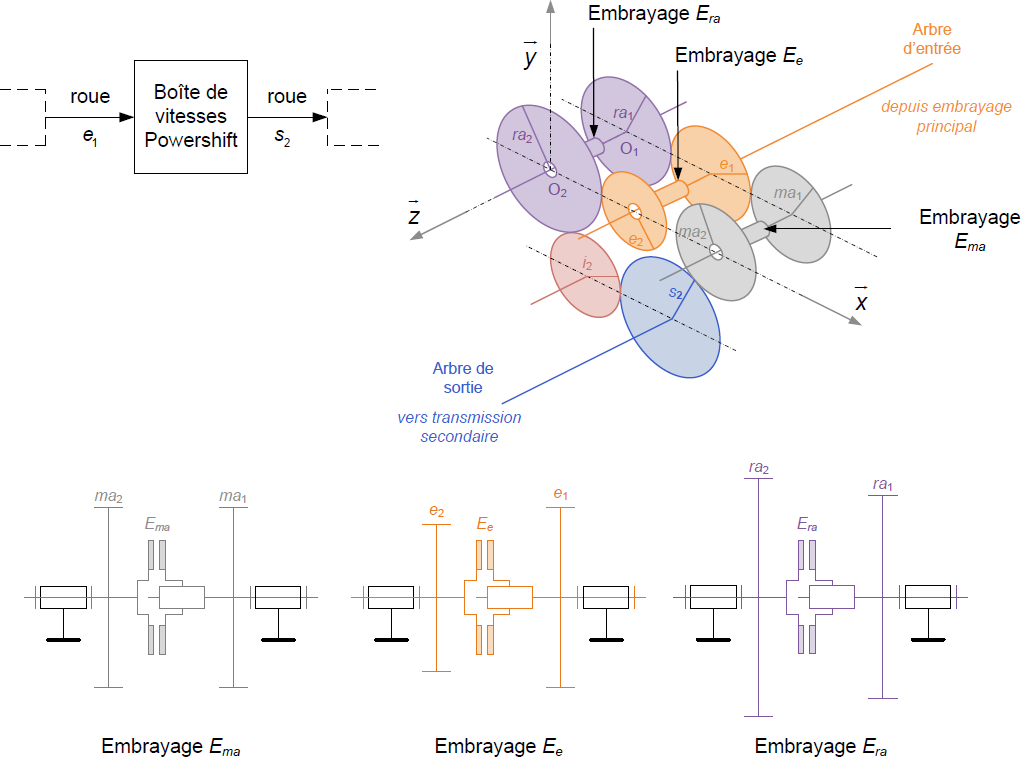
\includegraphics[width=.7\linewidth]{fig_18}
\caption{\label{fig_18} Schéma cinématique de l'unité de positionnement vertical (sur cette figure ($\theta_4 = 0\degres$))}
\end{figure}

La tête optique (non représentée sur ce schéma) sera fixée à la pièce (4).
Cette unité de positionnement vertical ($z$) est composée de deux sous-ensembles :
\begin{itemize}
\item un système quatre barres (0, 3, 4, 5). Ce système permet le déplacement selon ($z_0$) de la tête optique qui est solidaire de (4) ;
\item un système moteur (1, 2). L’axe de sortie du moteur couple est noté (1). La translation de la tête optique (4) est obtenue par la biellette (2) qui est liée à l’axe de sortie du moteur couple (en A) et à la pièce (3) en (F).
\end{itemize}
Ce mécanisme comporte cinq liaisons pivot (d’axe $\axe{O}{y_0}$, $\axe{B}{y_0}$, $\axe{C}{y_0}$, $\axe{D}{y_0}$, $\axe{E}{y_0}$) et deux liaisons qu’il convient de définir.

\textbf{Données : }
$\vect{OA}=l_1\vect{x_1}$, 
$\vect{FA}=l_2\vect{z_2}$, 
$\vect{CB}=l_3\vect{x_3}$, 
$\vect{CF}=l_3\vect{x_3} +b_3 \vect{z_3} $, 
$\vect{DE}=l_5\vect{x_5}$, 
$\vect{EB}=l_4\vect{z_4}$, 
$\vect{CD}=-f\vect{z_0}$, 
$\vect{OC}=d\vect{x_0}-e\vect{z_0}$, 
$\theta_1 = \angl{x_0}{x_1}$,
$\theta_2 = \angl{z_0}{z_2}$,
$\theta_3 = \angl{x_0}{x_3}$,
$\theta_4 = \angl{z_0}{z_4}$,
$\theta_5 = \angl{x_0}{x_5}$.
\fi

\subsubsection{Solution technique du système quatre barres}
\ifprof
\else
Dans un premier temps, nous étudierons le modèle quatre barres (0, 3, 4, 5) en cherchant à vérifier, que
cette nouvelle cinématique permet d’empêcher la rotation de la tête optique (en liaison encastrement avec
la pièce (4), puis à définir des solutions réelles pour les différentes liaisons.
\fi

\question{\label{q_16}Donnez la(les) relation(s) qu’il faut respecter entre les paramètres ($l_3$, $l_4$, $l_5$, $f$ ) pour que la tête
optique (fixée à (4)) n’ait aucun mouvement de rotation par rapport à (0). Vous justifierez
rapidement votre proposition.
Quelle est la nature du mouvement entre (4) et (0) ?}
\ifprof
\begin{corrige}
Pour que 4 n'ait aucun mouvement de rotation par rapport (0) il faut par exemple que (BE) et (CD) soient systèmatiquement parallèles. Pour cela, le quadrilatère (BCDE) doit être un parallélogramme et donc $l_4=f$ et $l_3=l_4$.

Le mouvement de (4) par rapport (0) est une translation ciruclaire. 
\end{corrige}
\else
\fi

\question{\label{q_17}Calculez la mobilité et le degré d’hyperstaticité de ce modèle du mécanisme (0, 3, 4, 5).
Commentez la valeur du degré d’hyperstaticité obtenu (avantages / inconvénients) pour le modèle du
mécanisme étudié dont la fonction est d’assurer un positionnement vertical.}
\ifprof
\begin{corrige}
Pour le système 4 barres  (0, 3, 4, 5) il y a une mobilité.

Il y a 4 liaisons pivot donc 4 inconnues cinématiques.

Ces 4 barres forment un cycle. Il y a donc 6 équations cinématiques. 

Au final, $h = m - I_c + E_c = 1-4+6 =3$.

Le modèle est donc hyperstatique, permettant une plus grande rigidité du mécanisme. Cela est préférable pour assurer la robustesse du mécanisme et éviter la rotation de la tête.
\end{corrige}
\else
\fi
\ifprof
\else
Le système de positionnement vertical du point focal doit, absolument, se faire sans jeu dans les liaisons.
Tout jeu dans les liaisons induirait automatiquement une erreur dans la position verticale réelle du point
focal.
\fi

\question{\label{q_18}Proposez une solution technique pour réaliser des liaisons pivot sans jeu.
Dessinez, à main levée, un schéma technique spatial représentant le système quatre barres avec ces
différentes solutions techniques pour les liaisons.}
\ifprof
\begin{corrige}
Chacune des liaisons pivot peut être assuré, par exemple par la réalisation d'une rotule et d'une linéaire annulaire...

\end{corrige}
\else
\fi

\subsubsection{Transmission du mouvement entre le moteur couple et la tête optique}
\ifprof
\else
La seconde partie du mécanisme est un transmetteur, qui permet le déplacement de la pièce (4) à partir du
mouvement de rotation du moteur couple.

Pour ce mécanisme, le concepteur a choisi une disposition géométrique particulière : en position de
référence, les angles $\theta_1$, $\theta_2$, $\theta_3$ et $\theta_4$ sont tous nuls.
\fi

\question{\label{q_19}Quelles sont les raisons qui ont conduit le concepteur de ce mécanisme à choisir cette disposition ?}
\ifprof
\begin{corrige}
...
\end{corrige}
\else
\fi

\ifprof
\else
On désire que le mécanisme (de transmission de mouvement) (0, 1, 2, 3) soit isostatique. On ne se
préoccupe pas, dans cette partie, de réaliser (bien que ce soit également nécessaire) un système sans jeu.
\fi

\question{\label{q_20}Proposez, en justifiant votre réponse, une solution (liaison 1 et liaison 2) permettant d’obtenir un
modèle de mécanisme (0, 1, 2, 3) isostatique.}
\ifprof
\begin{corrige}
Pour rendre le modèle isostatique, on peut par exemple utiliser des rotules à la place des liaisons 1 et 2. 
On aurait donc :
\begin{itemize}
\item $m=2$;
\item $I_c = 8$;
\item $E_c = 6$;
\item $h=2-8+6=0$ : modèle isostatique. 
\end{itemize}
\end{corrige}
\else
\fi